% Progetto di ingegneria del software - Relazione (pdf)

\documentclass[twoside,openright,titlepage,fleqn,headinclude,12pt,a4paper,BCOR=5mm,footinclude]{scrbook}

\usepackage{float}
\usepackage{placeins}
\usepackage{array}
\usepackage[nottoc]{tocbibind}
\usepackage[utf8]{inputenc} 
\usepackage[T1]{fontenc} 
\usepackage[english]{babel}
\usepackage{csquotes}
\usepackage[fleqn]{amsmath}  
\usepackage{ellipsis}
\usepackage{listings}
\usepackage{subfig}
\usepackage{caption}
\usepackage{appendix}
\usepackage{siunitx}
\usepackage[pdftex]{graphicx}
\usepackage[eulerchapternumbers,linedheaders,subfig,beramono,eulermath,parts,dottedtoc]{classicthesis}
\usepackage{geometry}

\newlength{\abcd} 
\setlength{\extrarowheight}{3pt} 
\captionsetup{format=hang,font=small}

\geometry{
	a4paper,
	ignoremp,
	bindingoffset = 1cm, 
	textwidth     = 13.5cm,
	textheight    = 21.5cm,
	lmargin       = 3.5cm, 
	tmargin       = 4cm    
}

\lstset{
  	frame=tb,
	language=Matlab,
  	aboveskip=3mm,
  	belowskip=3mm,
  	showstringspaces=false,
  	columns=flexible,
  	basicstyle={\small\ttfamily},
  	numbers=none,
  	breaklines=true,
  	breakatwhitespace=true,
  	tabsize=3
}

\begin{document}
\frenchspacing
\raggedbottom
\pagenumbering{roman}
\pagestyle{plain}

\begin{titlepage}
    \begin{center}
        \large
        \hfill        
        \vfill
        \begingroup
            \includegraphics[scale=0.15]{images/logo}\\
            Scuola di Ingegneria\xspace\\
            Corso di Laurea in Ingegneria Informatica\xspace\\
            \vspace{0.5cm}
            \vspace{0.5cm}
            \textbf{Progetto di Ingegneria del Software}\\
            \vspace{0.5cm}
        \endgroup
        \vfill
        \begingroup
        Applicazione per la gestione di prestiti bibliotecari \xspace \\ $\ $\\
	\bigskip
	\bigskip
      \endgroup
      \spacedlowsmallcaps{Bernacchioni Lapo, Fallani Cosimo \xspace}
      \vfill 
      \vfill
	\bigskip
	\bigskip
      \vfill
      \vfill
      \vfill
      \vfill
      \vfill
      \vfill
      \vfill
      \vfill
      Anno Accademico 2024-2025
	\end{center}        
\end{titlepage}   

\newpage
\thispagestyle{empty}
\hfill
\vfill
\noindent Bernacchioni Lapo, Fallani Cosimo \xspace: 
\textit{ Applicazione per la gestione di prestiti bibliotecari \xspace,} 
Ingegneria del Software \xspace, \textcopyright\ Anno Accademico 2024-2025 \xspace

\pagestyle{scrheadings}
\cleardoublepage
\clearpage
\pagenumbering{arabic}
\tableofcontents
\cleardoublepage

\clearpage
\chapter{Introduzione}

\section{Obiettivi del progetto}
Il presente progetto ha l’obiettivo di sviluppare un sistema di gestione delle prenotazioni per una biblioteca, consentendo agli utenti di effettuare prenotazioni, monitorare lo stato dei libri, prendere in prestito e restituire volumi in modo automatizzato ed efficiente. Il sistema si propone di ridurre il carico gestionale del personale bibliotecario, garantendo un'organizzazione chiara delle prenotazioni e un controllo dettagliato delle operazioni di prestito e restituzione.

Gli utenti registrati possono visualizzare la disponibilità dei libri, effettuare una prenotazione e monitorarne lo stato fino alla restituzione. Il sistema prevede inoltre un controllo sulle date di scadenza, consentendo di identificare prestiti scaduti e notificare gli utenti per la restituzione. Il personale bibliotecario ha la possibilità di gestire il catalogo, aggiornare lo stato dei libri, approvare prenotazioni e verificare la regolarità delle restituzioni.

L’architettura software è strutturata secondo il paradigma Model-View-Controller (MVC), garantendo una chiara separazione tra interfaccia utente, logica applicativa e gestione dei dati. Il sistema implementa il Data Access Object (DAO) Pattern, che assicura un accesso ai dati strutturato e indipendente dall’implementazione del database, facilitando eventuali future estensioni o migrazioni. 


\section{Elementi del progetto}

Il sistema di gestione delle prenotazioni per la biblioteca è strutturato attorno a tre entità principali: Utenti (User), libri (Item) e Prenotazioni (Reservation). Queste componenti interagiscono tra loro per garantire la corretta gestione del prestito e della restituzione dei libri.
\begin{itemize}
    \item \textbf{Utenti}: rappresenta una persona registrata nel sistema, che può assumere diversi ruoli:
        \begin{itemize}
            \item \textbf{User}: può effettuare prenotazioni, consultare lo stato dei propri prestiti e ricevere notifiche relative alle scadenze.
            
            \item \textbf{Staff}:  ha il compito di gestire e monitorare le prenotazioni attive, verificare le scadenze e registrare la restituzione dei libri. Può anche annullare prenotazioni in casi specifici e segnalare eventuali problemi legati ai prestiti.

            \item \textbf{Manager}:  è responsabile della gestione del catalogo, quindi può aggiungere, modificare o rimuovere libri dal sistema.
            
        \end{itemize}
    
    \item \textbf{Item}: rappresenta un libro o un altro materiale disponibile per il prestito. Ogni libro è identificato da un codice univoco e possiede informazioni come titolo, autore, genere e stato. 
    
    \item \textbf{Reservation}: è l'oggetto attraverso cui un utente richiede un libro in prestito. La prenotazione include informazioni come la data di inizio, la data di scadenza e lo stato attuale. Il sistema gestisce automaticamente la scadenza delle prenotazioni e notifica gli utenti in caso di ritardi o necessità di restituzione.
    
\end{itemize}

\section{Estendibilità del progetto}

Il progetto è stato concepito per essere facilmente estendibile, in particolare per quanto riguarda l’integrazione di nuove funzionalità relative alla gestione delle prenotazioni e al controllo del catalogo bibliotecario. Una delle principali possibilità di estensione riguarda l’aggiunta di nuove tipologie di materiali prenotabili, come e-book o audiolibri, che richiederebbero l’implementazione di un sistema di accesso digitale e gestione delle licenze.

Un’ulteriore espansione del sistema potrebbe includere la gestione delle prenotazioni interbibliotecarie, consentendo agli utenti di prenotare libri da più sedi collegate allo stesso database e implementando un sistema di trasferimento tra biblioteche. A questa estensione si collega anche la possibilità di visualizzare una disponibilità globale degli elementi, offrendo un sistema di ricerca avanzato che tenga conto delle copie disponibili in tutte le biblioteche della rete.

Infine una espansione necessaria sarebbe una interfaccia che permetta l'assegnazione dei ruoli a gli utenti nel database da parte dei manager.


\chapter{Analisi dei requisiti}
\section{Use Case Diagram}
Il software presenta tre diversi tipi di attori: l'Utente, lo Staff e il Manager, inoltre sono presenti delle funzioni per registrarsi o autenticarsi per i guest. L'Utente può effettuare prenotazioni, visualizzare la disponibilità dei libri e gestire i propri prestiti. Lo Staff si occupa della gestione delle prenotazioni,  confermando le richieste e registrando le restituzioni. Il Manager, invece, è responsabile della gestione del database, potendo aggiungere, modificare o rimuovere libri. Lo schema dei casi d’uso sottostante è stato realizzato mediante StarUML.

\begin{figure}[H]
  \centering
  \includegraphics[width=1\linewidth]{images/useCaseDiag.jpg}
  \caption{Use Case Diagram}
  \label{fig:Use Case Diagram}
\end{figure}

\section{Use Case Templates}


\subsection{Casi d’uso principali di uno User}

\begin{table}[H]
    \centering
    \begin{tabular}{|>{\raggedright\arraybackslash}m{2.5cm}|>{\raggedright\arraybackslash}m{10cm}|}
        \hline
        \textbf{UC-1} & \textbf{Prenotazione di un libro} \\
        \hline
        \textbf{Descrizione} & Lo user seleziona un libro disponibile dal catalogo e procede alla prenotazione. Il sistema associa il libro all’utente e ne aggiorna lo stato a "prenotato". \\
        \hline
        \textbf{Livello} & User goal \\
        \hline
        \textbf{Attore principale} & User \\
        \hline
        \textbf{Azioni} & 
        1. Lo user accede alla dashboard personale. \newline
        2. Visualizza l’elenco dei libri disponibili. \newline
        3. Seleziona un libro e conferma la prenotazione. \newline
        4. Il sistema crea la prenotazione, associa il libro all’utente e ne aggiorna lo stato a "prenotato". \\
        \hline
        \textbf{Casi straordinari} & 
        2a. Se sono stati impostati dei filtri di ricerca nella dashboard i libri visualizzati rispetteranno i filtri. \\
        \hline
    \end{tabular}
    \caption{Prenotazione di un libro da parte dello User}
    \label{tab:book_reservation}
\end{table}

\begin{table}[H]
    \centering
    \begin{tabular}{|>{\raggedright\arraybackslash}m{2.5cm}|>{\raggedright\arraybackslash}m{10cm}|}
        \hline
        \textbf{UC-2} & \textbf{Annulla prenotazione di un libro} \\
        \hline
        \textbf{Descrizione} & Lo user può annullare una prenotazione effettuata in precedenza. Il sistema elimina la prenotazione associata e rende nuovamente disponibile il libro. \\
        \hline
        \textbf{Livello} & User goal \\
        \hline
        \textbf{Attore principale} & User \\
        \hline
        \textbf{Azioni} & 
        1. Lo user accede alla dashboard personale. \newline
        2. Visualizza l’elenco delle prenotazioni attive. \newline
        3. Seleziona la prenotazione da annullare. \newline
        4. Il sistema elimina la prenotazione e aggiorna lo stato del libro a "disponibile", se la prenotazione non è ancora attiva. \\
        \hline
        \textbf{Casi straordinari} & 
        4a. Se la prenotazione è già attiva (il libro è stato consegnato all’utente), il sistema non consente l’annullamento. \\
        \hline
    \end{tabular}
    \caption{Annullamento di una prenotazione da parte dello User}
    \label{tab:cancel_reservation}
\end{table}


\subsection{Casi d’uso principali degli staffer}

\begin{table}[H]
    \centering
    \begin{tabular}{|>{\raggedright\arraybackslash}m{2.5cm}|>{\raggedright\arraybackslash}m{10cm}|}
        \hline
        \textbf{UC-3} & \textbf{Conferma ritiro di un libro} \\
        \hline
        \textbf{Descrizione} & Lo staff conferma l'effettivo ritiro del libro da parte dell'utente, attivando ufficialmente la prenotazione. Il sistema registra l'inizio del periodo di prestito. \\
        \hline
        \textbf{Livello} & User goal \\
        \hline
        \textbf{Attore principale} & Staff \\
        \hline
        \textbf{Azioni} & 
        1. Lo staff accede alla dashboard dedicata. \newline
        2. Seleziona l’utente che ha effettuato la prenotazione. \newline
        3. Visualizza l’elenco delle prenotazioni gia attive, di quelle non ancora attive e di quelle concluse .\newline
        4. Clicca sul bottone dedicato relativo alla prenotazione da attivare. \newline
        5. Il sistema registra l’inizio della prenotazione e imposta lo stato su "attiva". \\
        \hline
        \textbf{Casi straordinari} & 
        4a. Se la prenotazione è già attiva o risulta scaduta, il sistema non consente l’attivazione. In tal caso il bottone é disattivato.  \\
        \hline
    \end{tabular}
    \caption{Conferma del ritiro di un libro da parte dello Staff}
    \label{tab:confirm_pickup}
\end{table}

\begin{table}[H]
    \centering
    \begin{tabular}{|>{\raggedright\arraybackslash}m{2.5cm}|>{\raggedright\arraybackslash}m{10cm}|}
        \hline
        \textbf{UC-4} & \textbf{Avvenuta restituzione di un libro} \\
        \hline
        \textbf{Descrizione} & Lo staff registra la restituzione del libro da parte dell’utente. Il sistema chiude la prenotazione e rende nuovamente disponibile il libro. \\
        \hline
        \textbf{Livello} & User goal \\
        \hline
        \textbf{Attore principale} & Staff \\
        \hline
        \textbf{Azioni} & 
        1. Lo staff accede alla dashboard dedicata. \newline
        2. Seleziona l’utente che ha effettuato la prenotazione. \newline
        3. Visualizza l’elenco delle prenotazioni gia attive, di quelle non ancora attive e di quelle concluse .\newline
        4. Clicca sul bottone dedicato relativo alla prenotazione da chiudere. \newline
        5. Il sistema disattiva la prenotazione e imposta lo stato del libro su "disponibile". \\
        \hline
        \textbf{Casi straordinari} & 
        4a. Se la prenotazione non è già attiva o é ancora in corso, il sistema non consente la chiusura. In tal caso il bottone é disattivato.  \\
        \hline
    \end{tabular}
    \caption{Registrazione della restituzione di un libro da parte dello Staff}
    \label{tab:book_return}
\end{table}


\subsection{Casi d’uso principali dei manager}

\begin{table}[H]
    \centering
    \begin{tabular}{|>{\raggedright\arraybackslash}m{2.5cm}|>{\raggedright\arraybackslash}m{10cm}|}
        \hline
        \textbf{UC-5} & \textbf{Aggiunta di un libro al database} \\
        \hline
        \textbf{Descrizione} & Il manager inserisce un nuovo libro nel catalogo della biblioteca compilando i campi richiesti. Il sistema salva il libro nel database rendendolo disponibile alla prenotazione. \\
        \hline
        \textbf{Livello} & User goal \\
        \hline
        \textbf{Attore principale} & Manager \\
        \hline
        \textbf{Azioni} & 
        1. Il manager accede alla dashboard di gestione. \newline
        2. Compila il modulo di inserimento con i dati del libro (titolo, autore, genere, tipo). \newline
        3. Conferma l’operazione. \newline
        4. Il sistema salva il libro nel database e lo rende disponibile per la prenotazione. \\
        \hline
        \textbf{Casi straordinari} & 
        2a. Se sono assenti dei dati obbligatori non é consentita la creazione del libro. \\
        \hline
    \end{tabular}
    \caption{Aggiunta di un libro al database da parte del Manager}
    \label{tab:add_book}
\end{table}

\begin{table}[H]
    \centering
    \begin{tabular}{|>{\raggedright\arraybackslash}m{2.5cm}|>{\raggedright\arraybackslash}m{10cm}|}
        \hline
        \textbf{UC-6} & \textbf{Rimozione di un libro dal database} \\
        \hline
        \textbf{Descrizione} & Il manager può rimuovere un libro dal catalogo della biblioteca. Il sistema elimina il libro dal database e lo rende non più disponibile alla prenotazione. \\
        \hline
        \textbf{Livello} & User goal \\
        \hline
        \textbf{Attore principale} & Manager \\
        \hline
        \textbf{Azioni} & 
        1. Il manager accede alla dashboard di gestione. \newline
        2. Visualizza l’elenco dei libri presenti nel catalogo. \newline
        3. Seleziona il libro da rimuovere. \newline
        4. Il sistema elimina il libro dal database. \\
        \hline
        \textbf{Casi straordinari} & 
        \\
        \hline
    \end{tabular}
    \caption{Rimozione di un libro dal database da parte del Manager}
    \label{tab:remove_book}
\end{table}

\begin{table}[H]
    \centering
    \begin{tabular}{|>{\raggedright\arraybackslash}m{2.5cm}|>{\raggedright\arraybackslash}m{10cm}|}
        \hline
        \textbf{UC-7} & \textbf{Modifica di un libro nel database} \\
        \hline
        \textbf{Descrizione} & Il manager può aggiornare le informazioni di un libro presente nel catalogo, modificando titolo, autore o genere. Il sistema salva le nuove informazioni nel database. \\
        \hline
        \textbf{Livello} & User goal \\
        \hline
        \textbf{Attore principale} & Manager \\
        \hline
        \textbf{Azioni} & 
        1. Il manager accede alla dashboard di gestione. \newline
        2. Visualizza l’elenco dei libri presenti nel catalogo. \newline
        3. Seleziona il libro da modificare. \newline
        4. Inserisce i nuovi dati nel modulo di modifica. \newline
        5. Conferma le modifiche. \newline
        6. Il sistema aggiorna le informazioni del libro nel database. \\
        \hline
        \textbf{Casi straordinari} & 
        5a. Se sono assenti dei dati obbligatori non é consentita la modifica del libro. \\
 \\
        \hline
    \end{tabular}
    \caption{Modifica di un libro nel database da parte del Manager}
    \label{tab:edit_book}
\end{table}



\section{Mockups}
Ecco alcuni Mockups che sono veri e propri screenshot della GUI realizzata a questo proposito.

\begin{figure}[H]
  \centering
  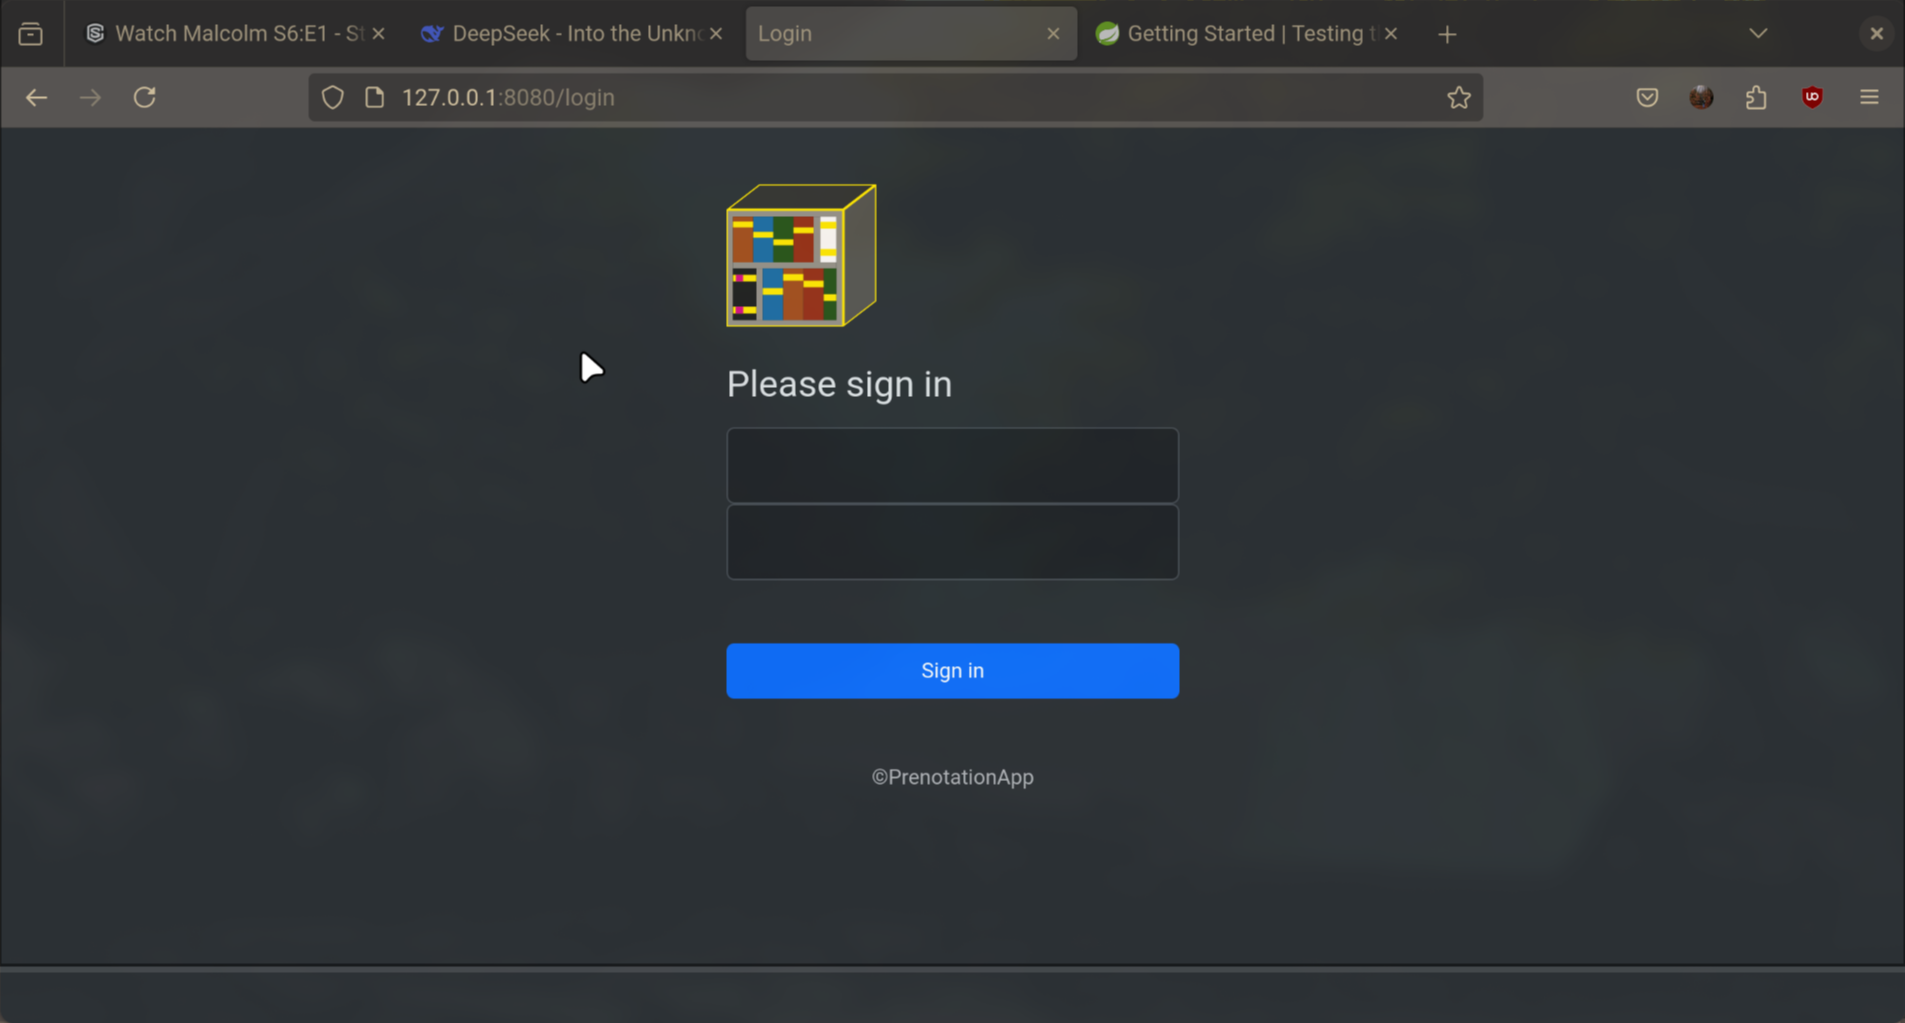
\includegraphics[width=0.9\linewidth]{images/Login.png}
  \caption{Pagina di login}
  \label{fig:Pagina di login}
\end{figure}
\begin{figure}[H]
  \centering
  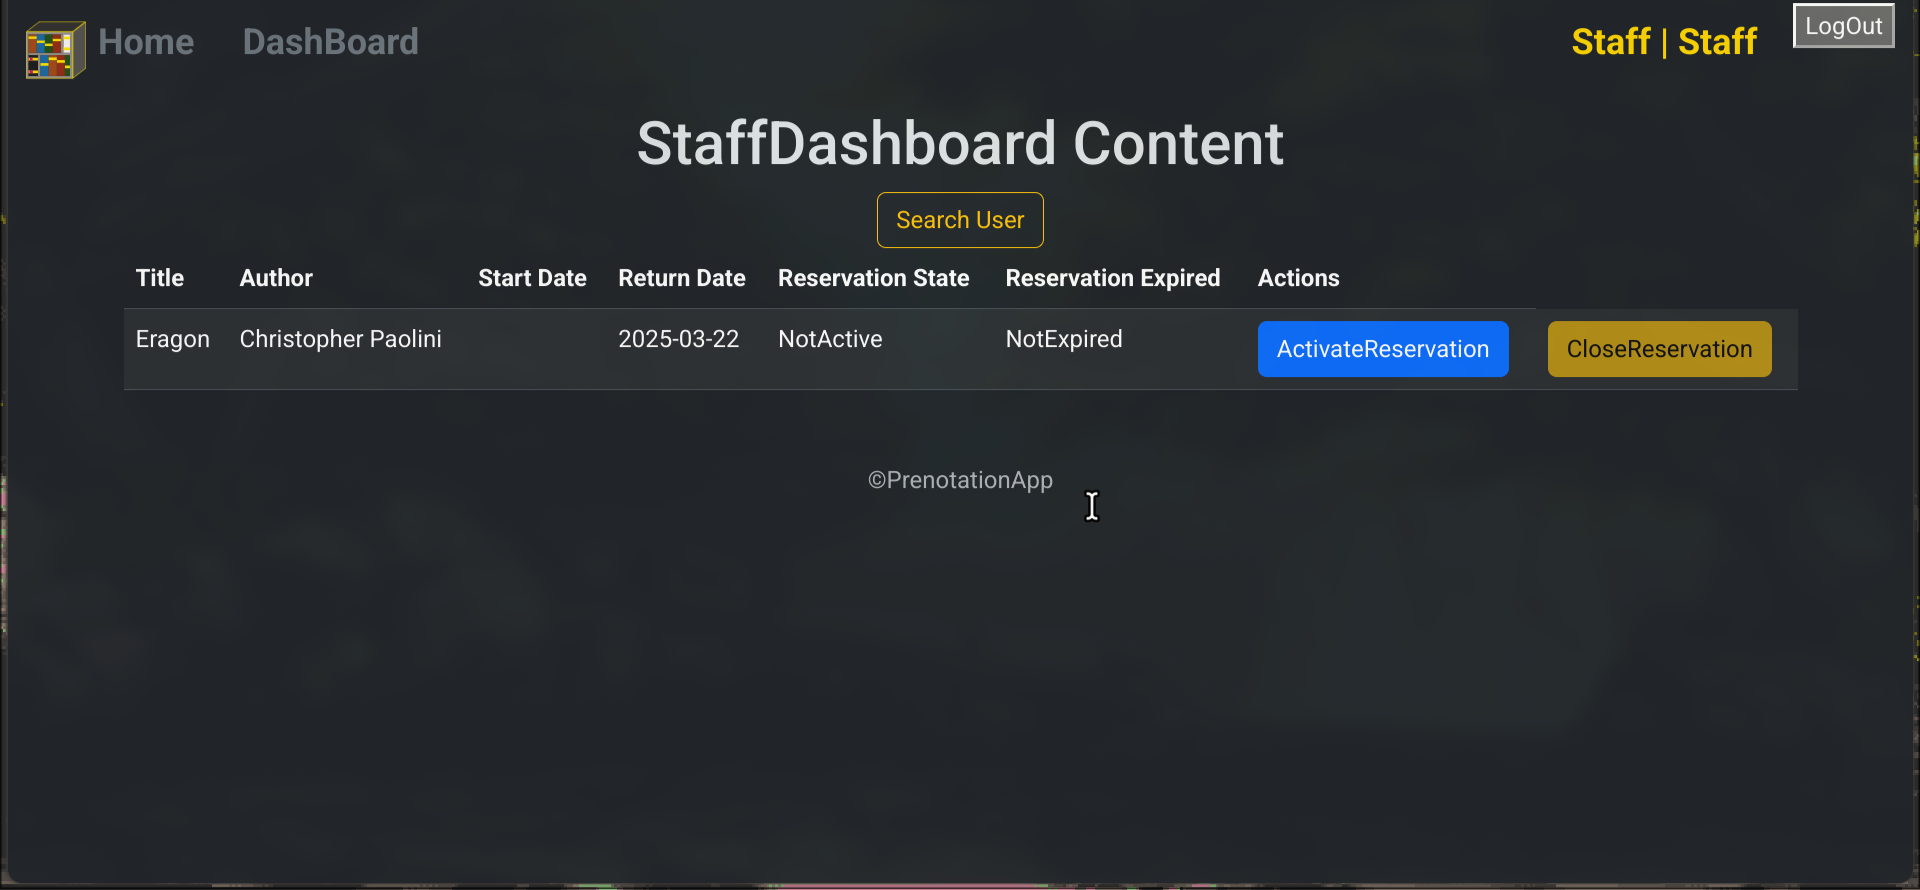
\includegraphics[width=0.9\linewidth]{images/StaffDashboard.png}
  \caption{Dashboard dello staff}
  \label{fig:Dashboard dello staff}
\end{figure}
\begin{figure}[H]
  \centering
  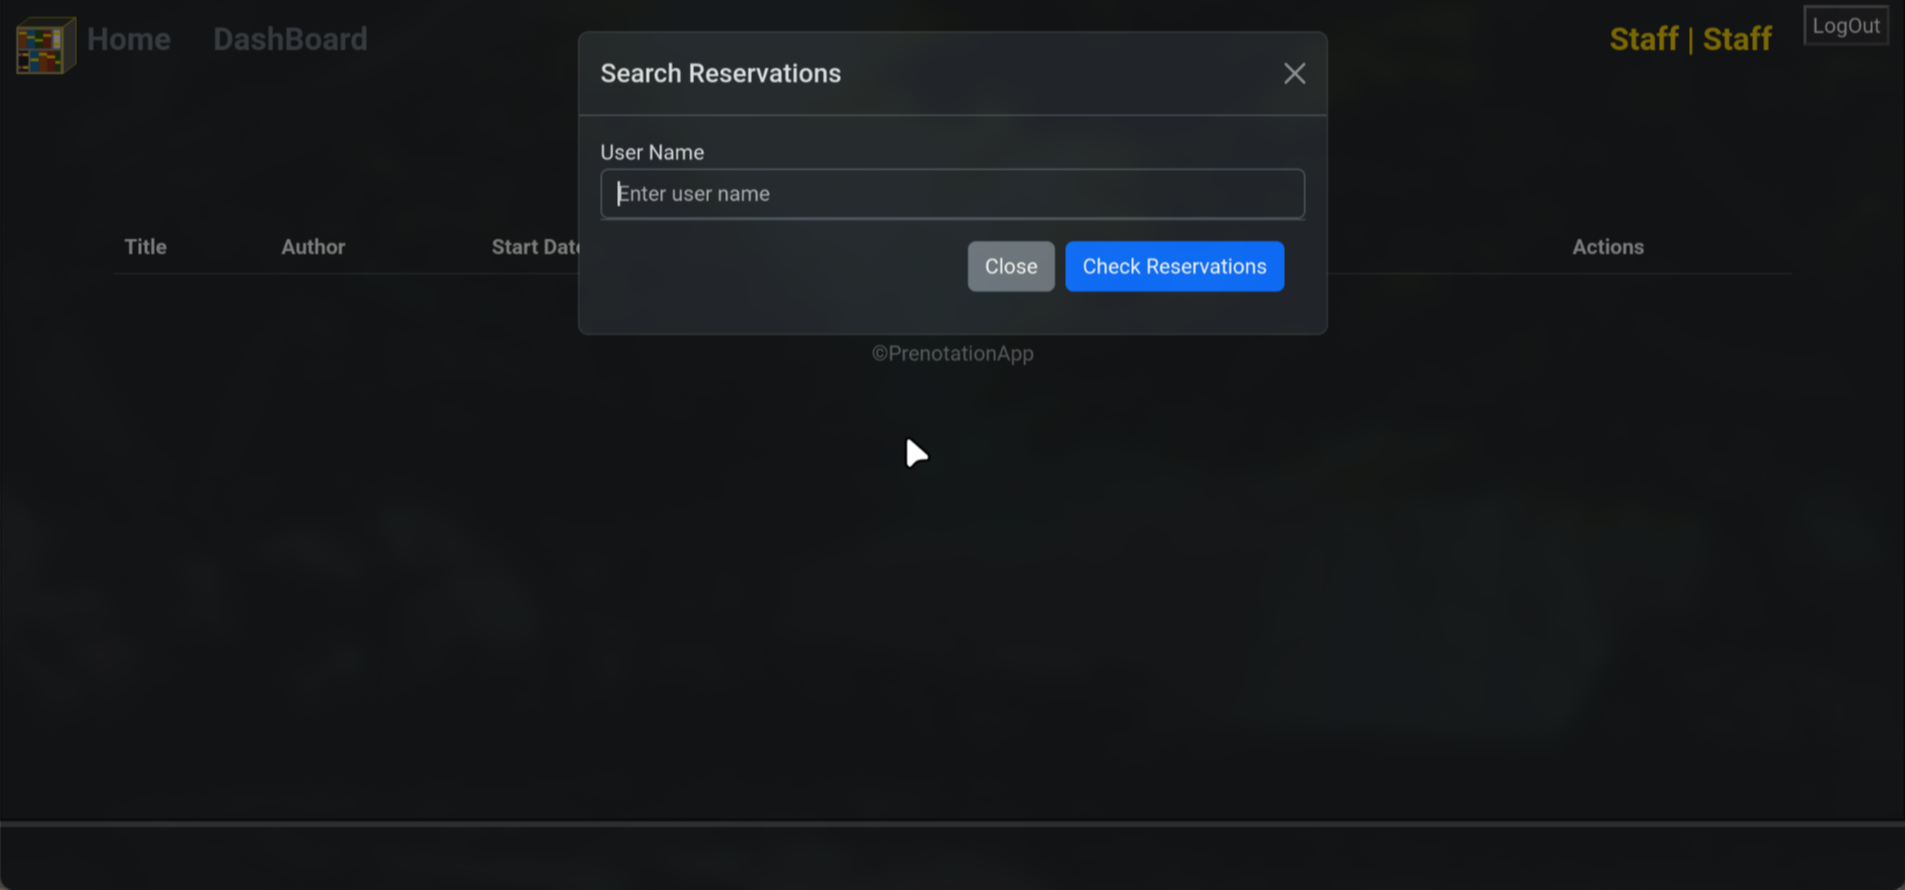
\includegraphics[width=0.9\linewidth]{images/SearchReservations.png}
  \caption{Barra di ricerca per l'attivazione dei prestiti}
  \label{fig:Barra di ricerca per l'attivazione dei prestiti}
\end{figure}
\begin{figure}[H]
  \centering
  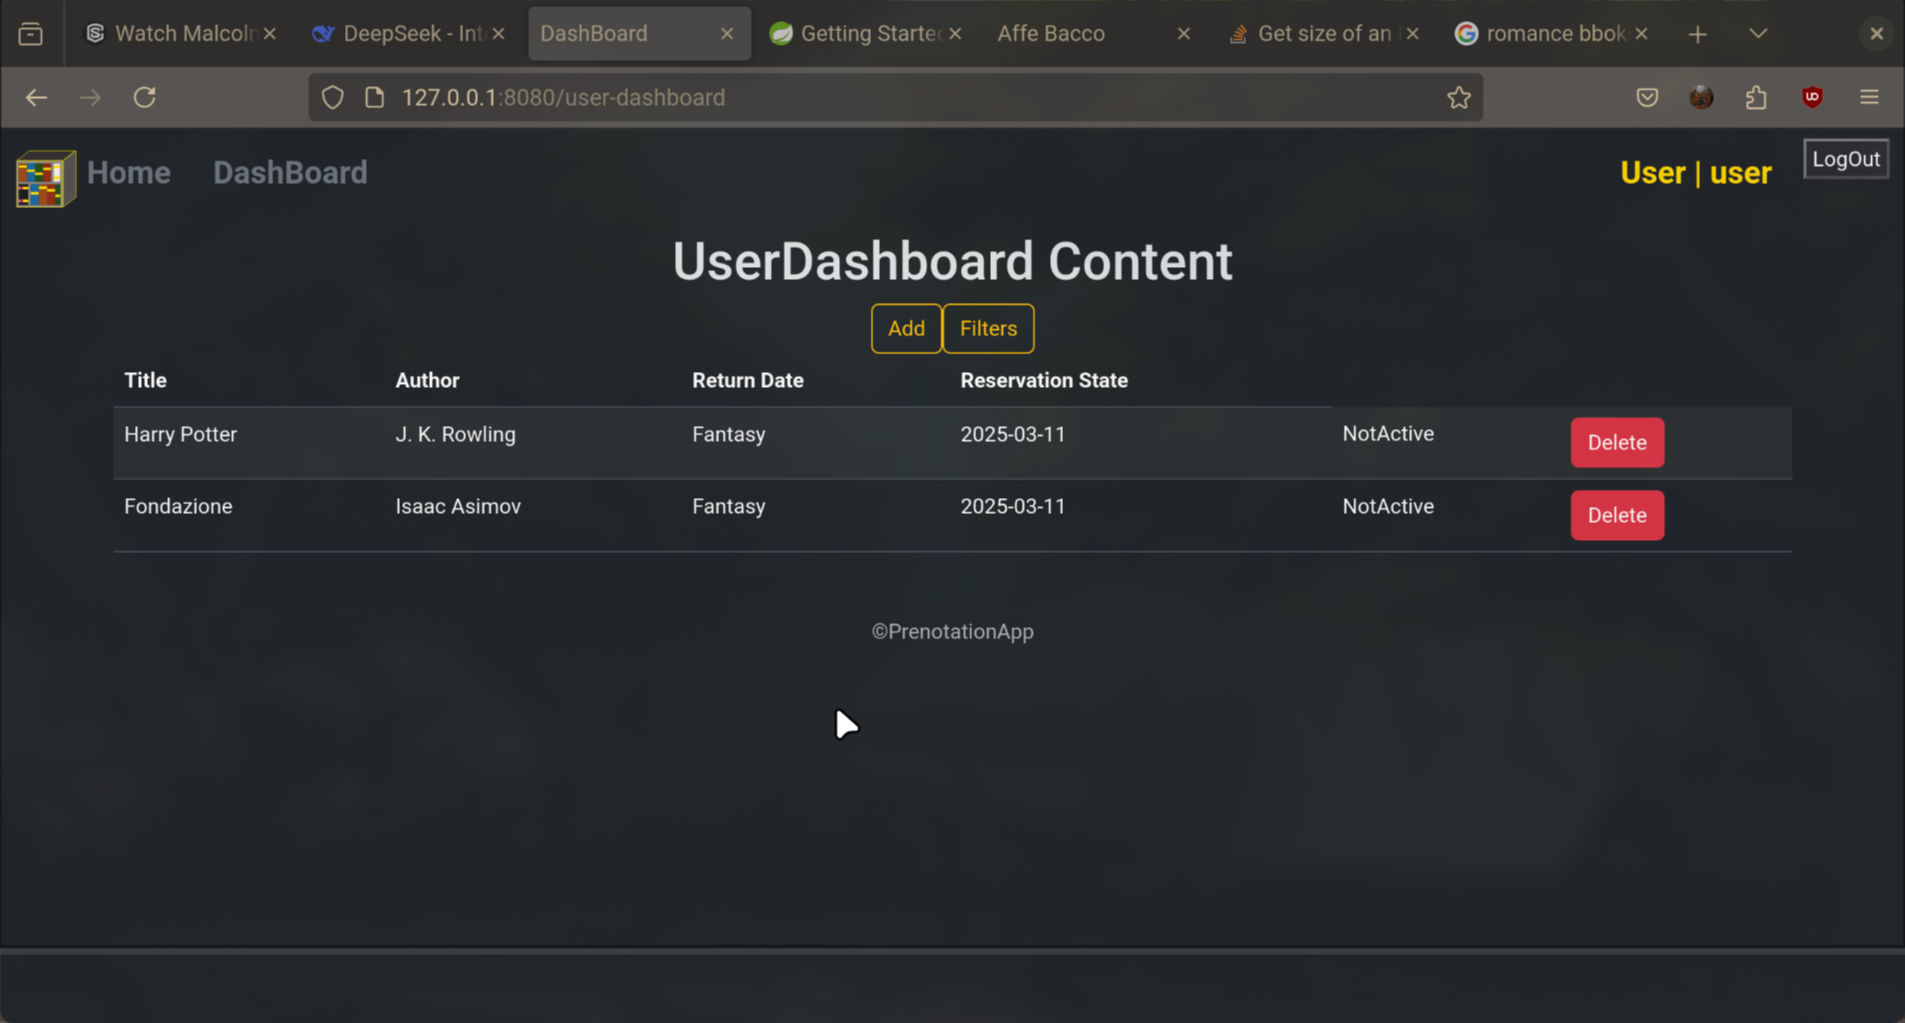
\includegraphics[width=0.9\linewidth]{images/UserDashboard.png}
  \caption{Dashboard degli utenti}
  \label{fig:Dashboard degli utenti }
\end{figure}
\begin{figure}[H]
  \centering
  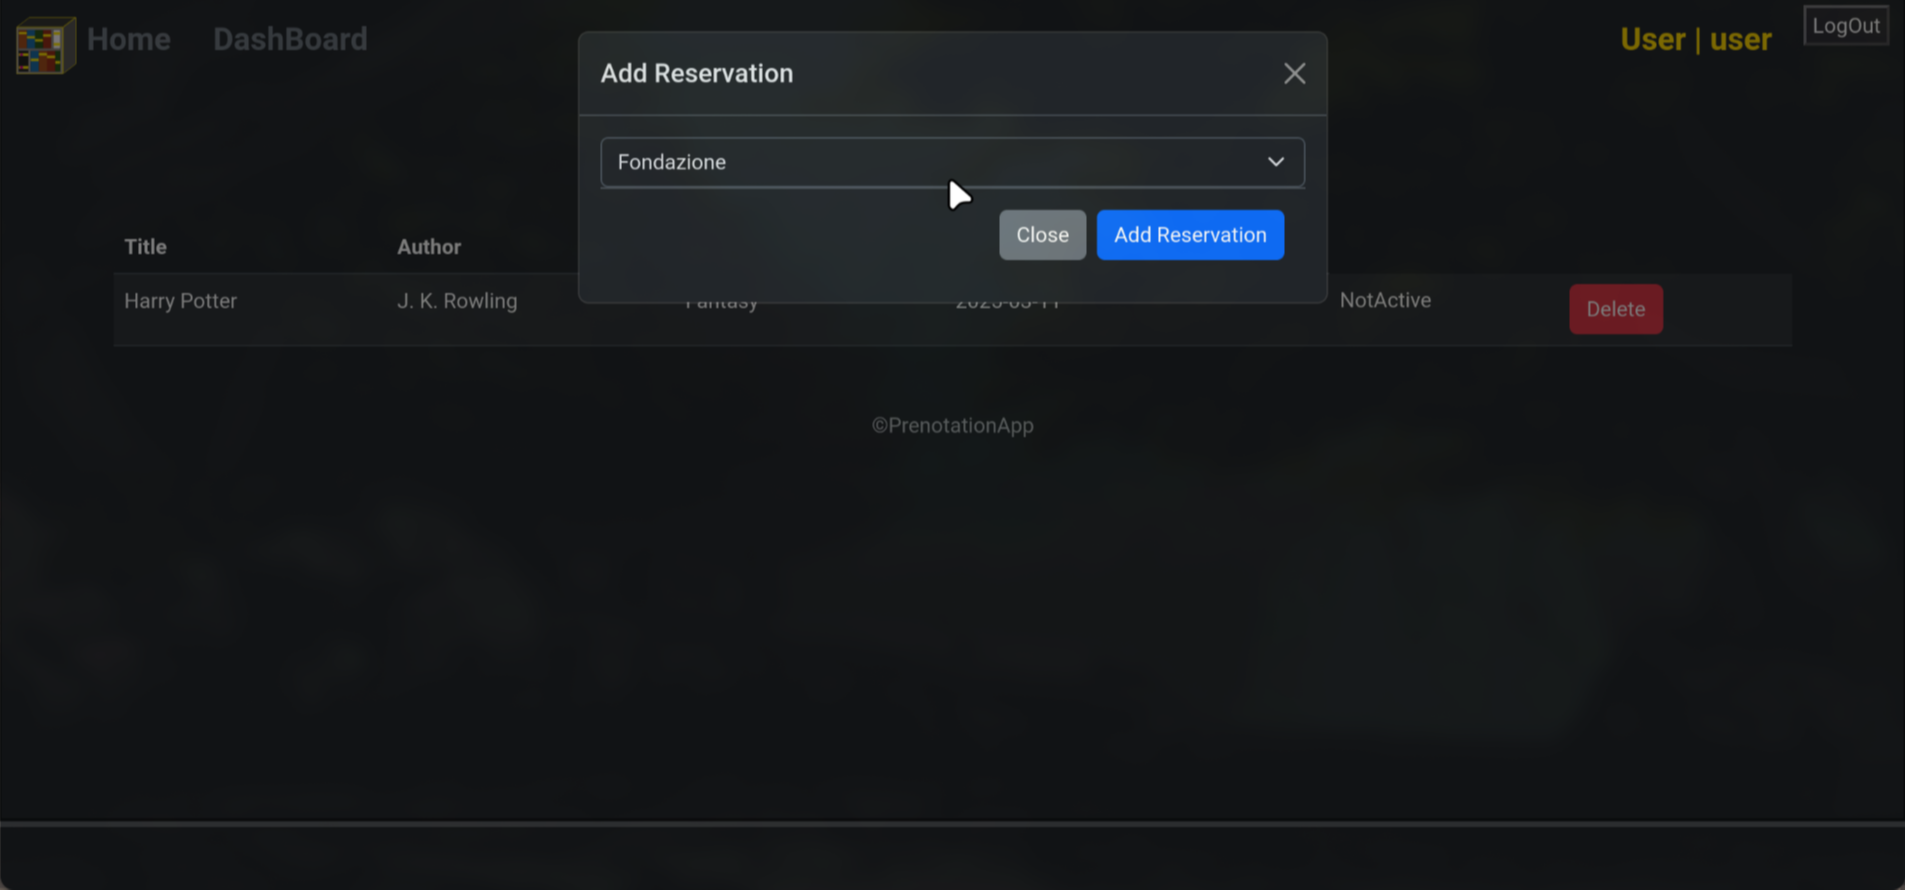
\includegraphics[width=0.9\linewidth]{images/AddReservation.png}
  \caption{Aggiunta di una prenotazione}
  \label{fig:Aggiunta di una prenotazione}
\end{figure}
\begin{figure}[H]
  \centering
  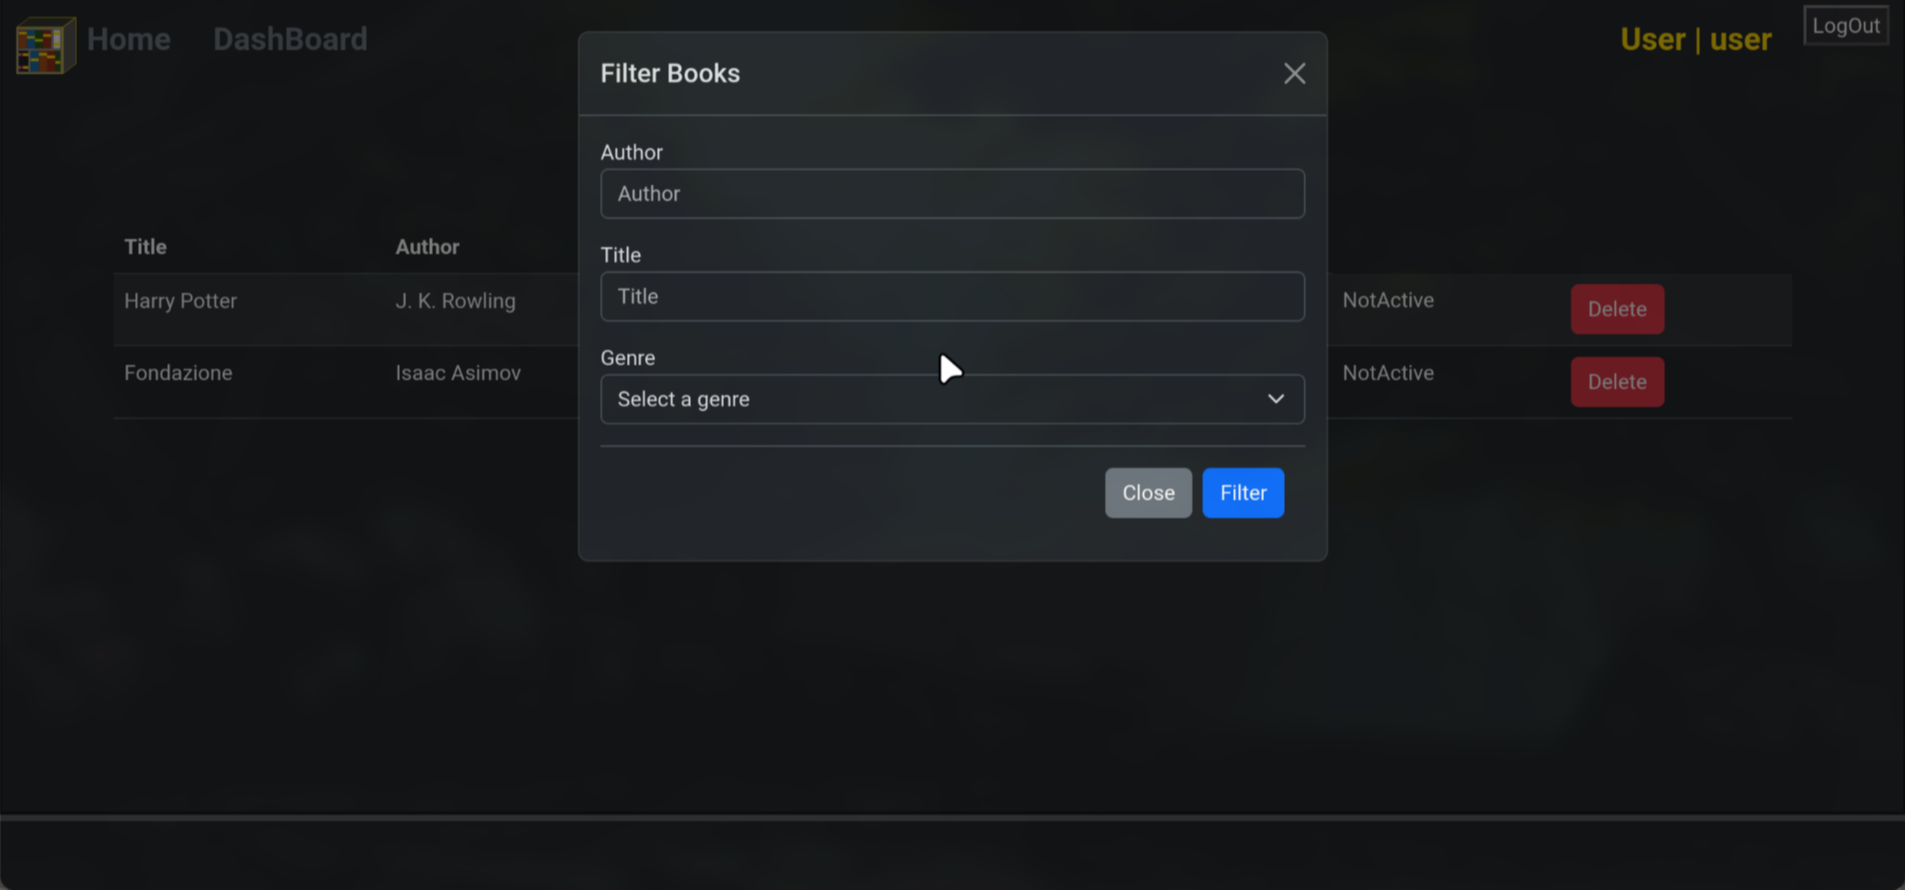
\includegraphics[width=0.9\linewidth]{images/FilterBook.png}
  \caption{Form per il filtraggio dei libri}
  \label{fig:Form per il filtraggio dei libri}
\end{figure}
\begin{figure}[H]
  \centering
  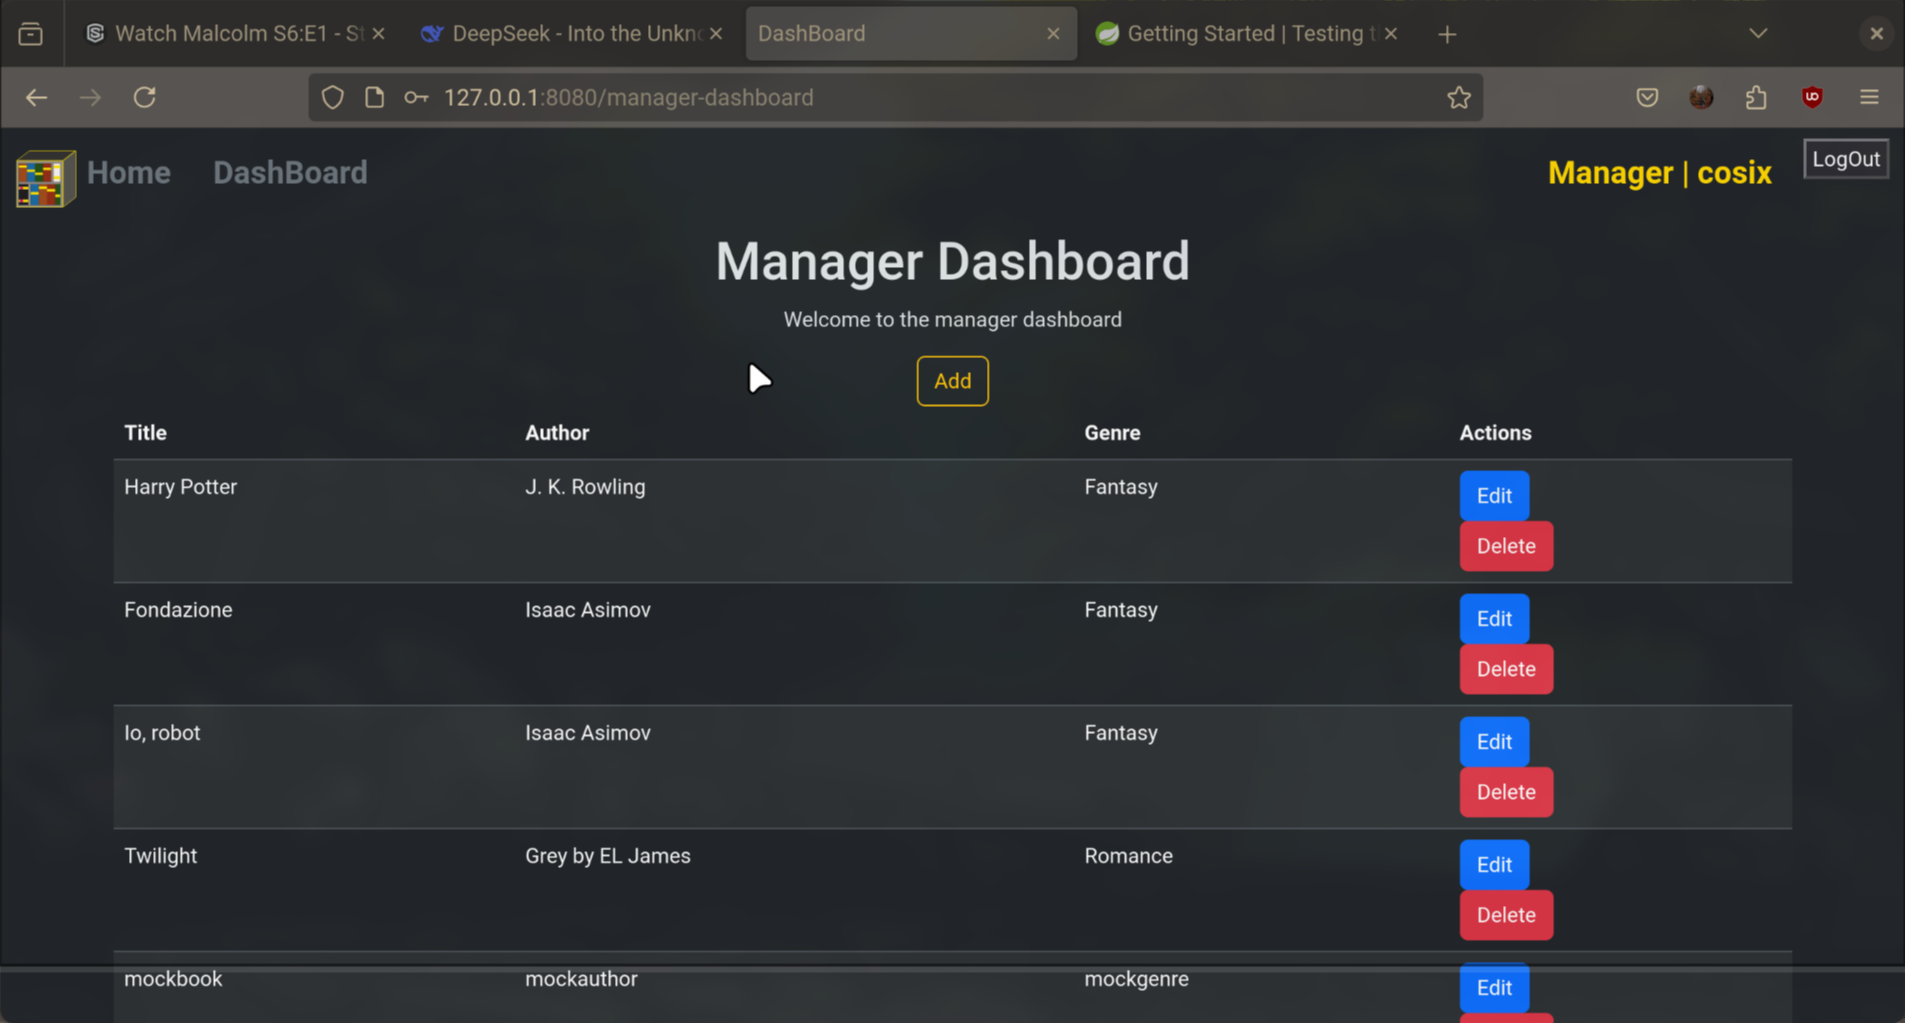
\includegraphics[width=0.9\linewidth]{images/ManagerDashboard.png}
  \caption{Dashboard del manager}
  \label{fig:Dashboard del manager}
\end{figure}
\begin{figure}[H]
  \centering
  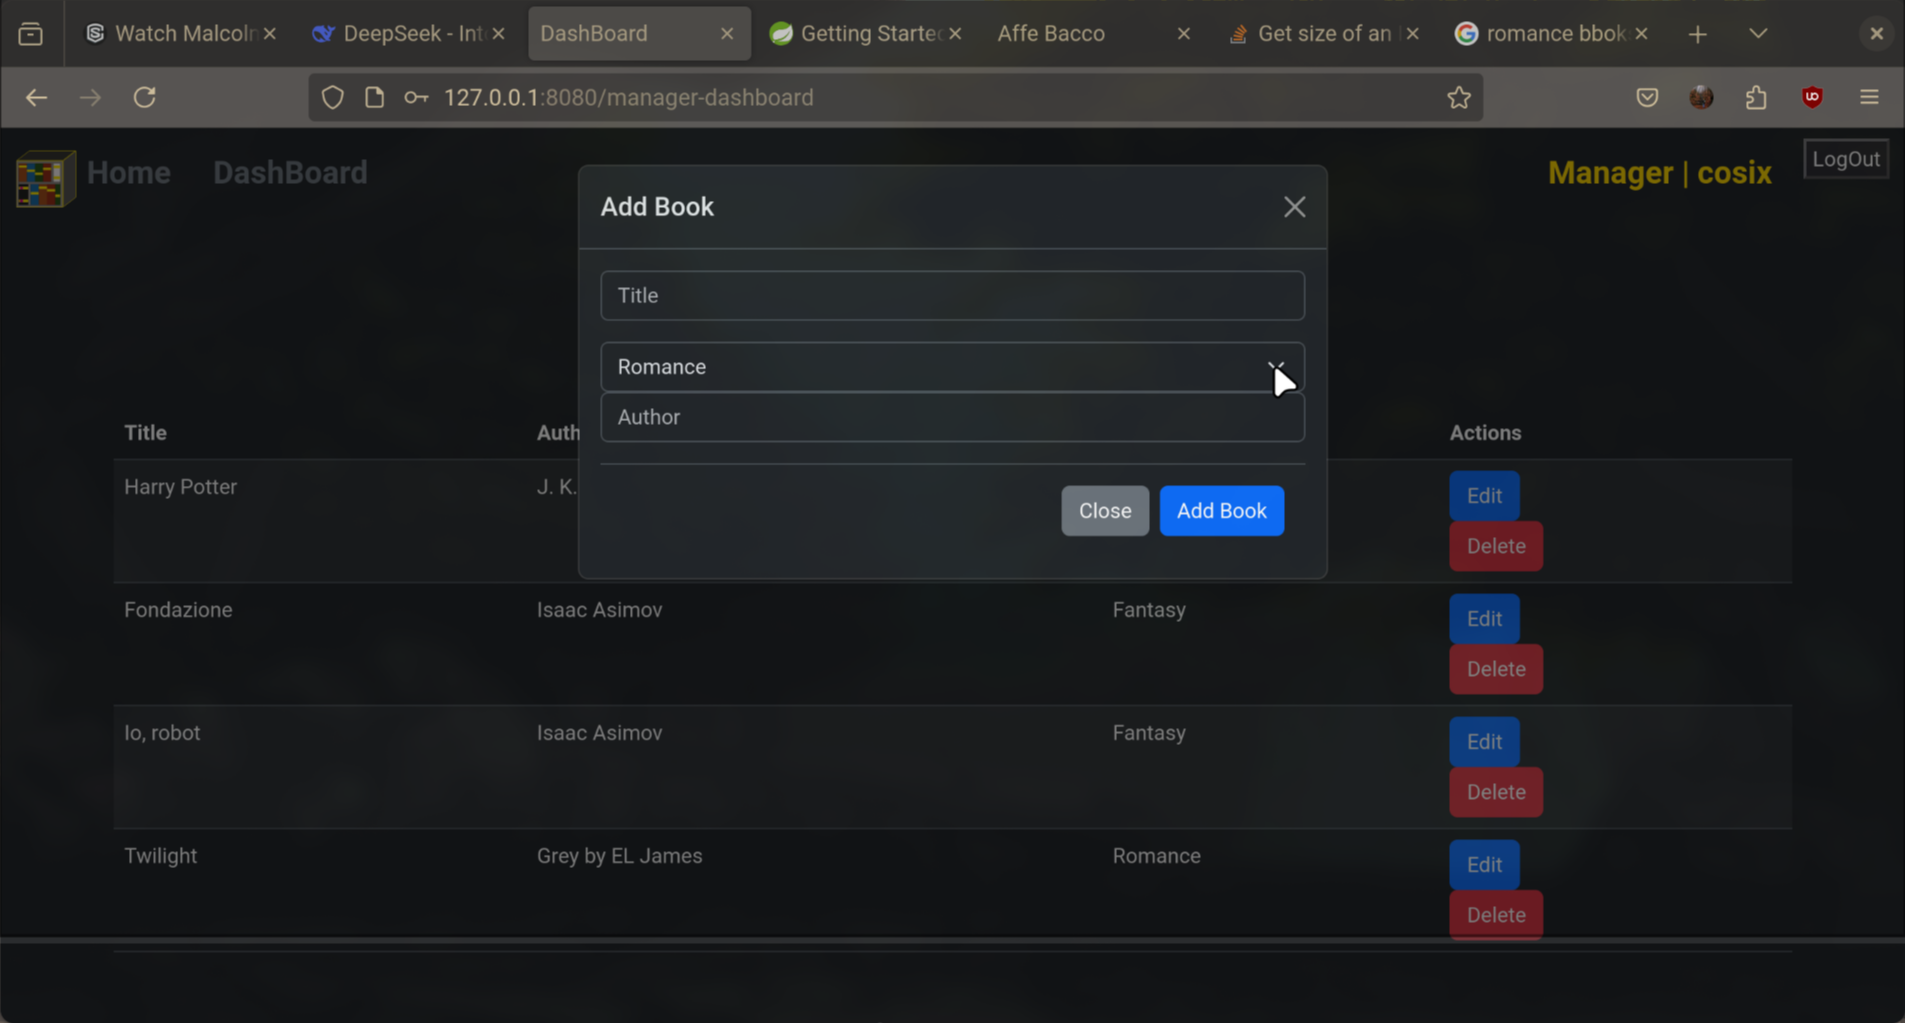
\includegraphics[width=0.9\linewidth]{images/AddBook.png}
  \caption{Form per l'aggiunta di un libro}
  \label{fig:Form per l'aggiunta di un libro}
\end{figure}
\begin{figure}[H]
  \centering
  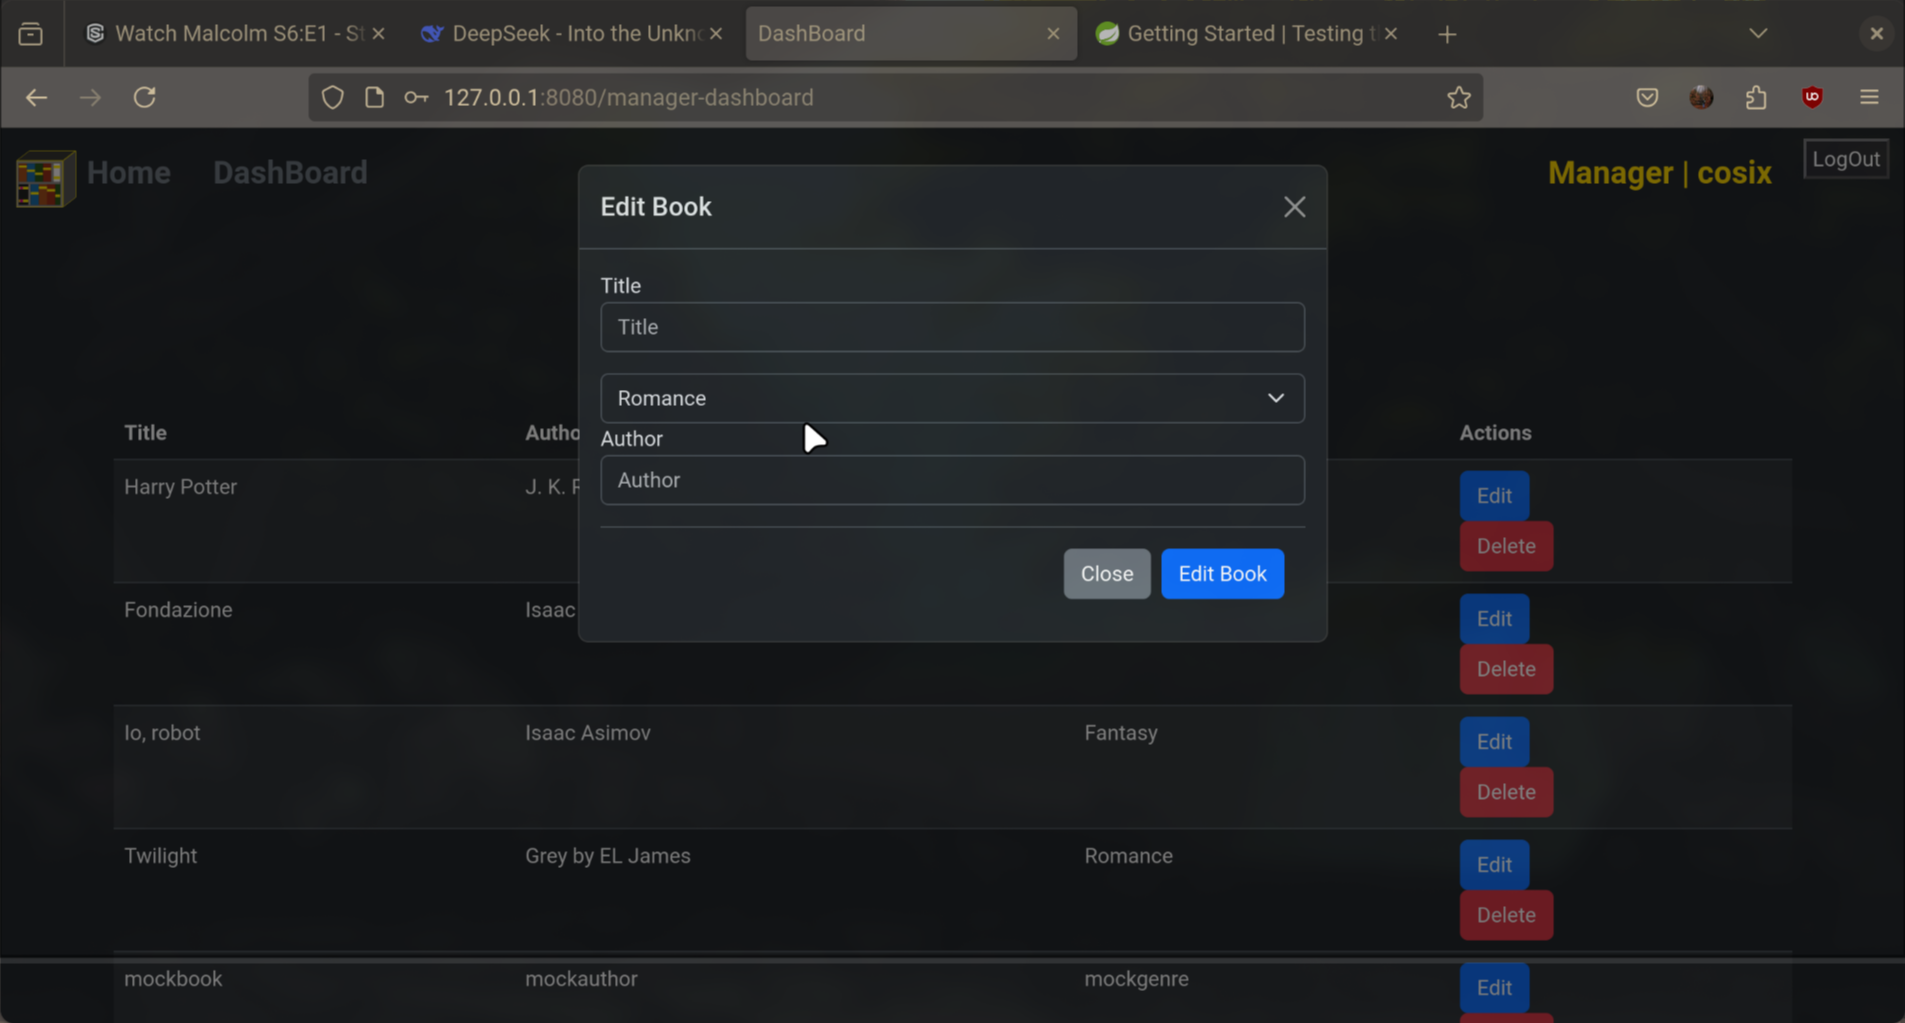
\includegraphics[width=0.9\linewidth]{images/EditBook.png}
  \caption{Form per la modifica di un libro}
  \label{fig:Form per la modifica di un libro}
\end{figure}

\section{Class Diagram}


\begin{figure}[H]
  \centering
  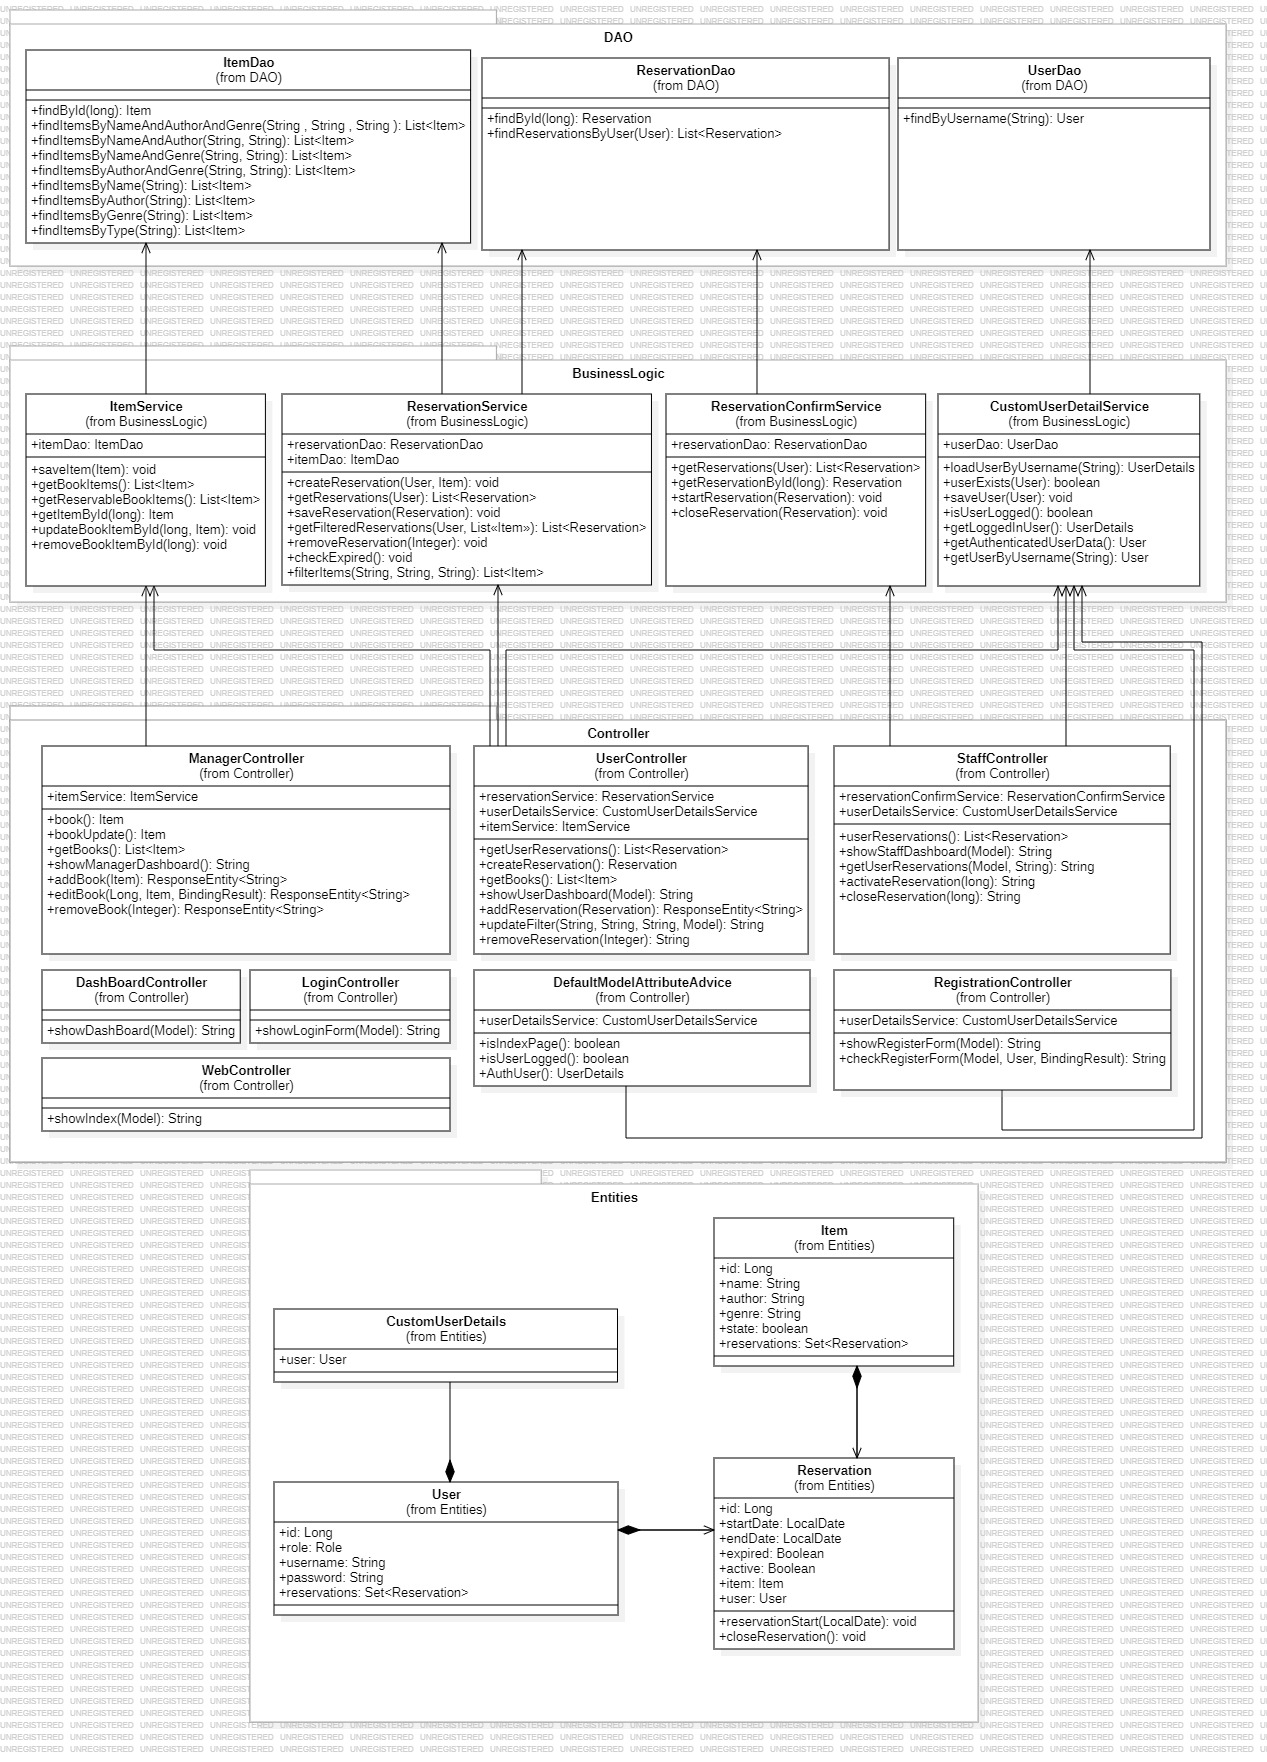
\includegraphics[width=1\linewidth]{images/classDiag.jpg}
  \caption{Use Case Diagram}
  \label{fig:Use Case Diagram}
\end{figure}

Il codice del sistema è organizzato in diversi package, ognuno con responsabilità specifiche per garantire modularità, separazione dei task e manutenibilità del software. Il Class Diagram evidenzia la suddivisione del software nei livelli DAO, Business Logic, Controller e Entities.
\begin{itemize}
    \item Entities: definisce le entità fondamentali del sistema, rappresentando gli oggetti principali come utenti, oggetti e prenotazioni. Ogni entità è modellata con attributi e relazioni che ne descrivono il comportamento all'interno del sistema.
    \item Business Logic: implementa la logica applicativa del sistema, fungendo da livello intermedio tra il DAO e i controller. Qui vengono definite le operazioni fondamentali come la gestione delle prenotazioni, l’elaborazione delle richieste e l’autenticazione degli utenti.
    \item DAO: fornisce le interfacce per l’accesso ai dati, consentendo di isolare la logica di persistenza e garantendo un’interazione efficiente con il database. Questo package include operazioni di ricerca, recupero e gestione di utenti, prenotazioni e libri.
    \item Controller : gestisce l’interazione con l’utente, elaborando le richieste e restituendo risposte appropriate. I controller si occupano delle richieste ai servizi offerti dal package buisness logic, come prenotazioni e modifica del catalogo bibliotecario.
   
\end{itemize} 
È importante sottolineare che le classi presenti nel package DAO non rappresentano un’implementazione tradizionale del DAO Pattern, ma fungono da wrapper per le funzionalità di accesso ai dati fornite da Spring Boot. Poiché il framework offre già un'astrazione per la gestione del database, le nostre classi DAO sono state progettate per migliorare la separazione delle responsabilità e garantire una maggiore chiarezza strutturale. L’adozione di questo approccio consente di mantenere un'architettura modulare e facilita eventuali modifiche future.




\section{DAO Pattern}

Abbiamo utilizzato il Design Pattern \textbf{DAO} (Data Access Object) per garantire che il client non possa interagire direttamente con il database.

Il pattern architetturale \textbf{DAO} viene impiegato per gestire la persistenza dei dati registrati nel database. La persistenza si riferisce alla capacità di un dato di "sopravvivere" all'esecuzione di un programma, mantenendo la coerenza anche dopo la terminazione del software. Questo pattern ha lo scopo di separare la logica di accesso ai dati dal resto dell’applicazione, isolando il codice responsabile della manipolazione dei dati da quello che implementa la logica di elaborazione.

Nel nostro progetto, il DAO definisce e offre metodi CRUD (Create, Read, Update, Delete) per la gestione dei dati nel database. Le principali classi che sfruttano il DAO e che sono presenti nel database sono le seguenti:

\begin{itemize}
    \item \textbf{UserDAO} → rappresenta gli utenti del sistema con i relativi dati di autenticazione e ruolo;
    \item \textbf{ItemDAO} → rappresenta gli oggetti disponibili per il prestito;
    \item \textbf{ReservationDAO} → gestisce le prenotazioni effettuate dagli utenti sui libri disponibili.
\end{itemize}


\section{MVC Pattern}
 Il pattern \textbf{MVC} è un'architettura software che separa i dati (\textbf{Model}), l’interfaccia utente (\textbf{View}) e la logica di controllo (\textbf{Controller}), garantendo una netta separazione delle responsabilità. 

Nel caso del nostro sistema, la suddivisione del pattern \textbf{MVC} è la seguente:
\begin{itemize}
    \item Il \textbf{Model} è rappresentato dalle classi presenti nel package \texttt{entities}, che definiscono i dati memorizzati nel database.
    \item La \textbf{View} corrisponde alle pagine HTML e alle risorse dell’interfaccia utente con cui l’utente interagisce.
    \item Il \textbf{Controller} è implementato nelle classi del package \texttt{controller}, che gestiscono le richieste dell'utente e tramite i servizi offerti dal package buisness logic aggiorna il modello di dati attraverso il pattern DAO.
\end{itemize}


\section{Entity Relationship Diagram}
Questo è il diagramma ER del progetto, con le varie cardinalità delle
relazioni.

\begin{figure}[H]
  \centering
  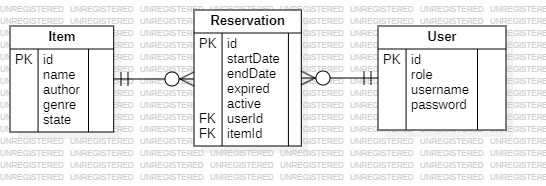
\includegraphics[width=1\linewidth]{images/relationsDiag.jpg}
  \caption{Use Case Diagram}
  \label{fig:Use Case Diagram}
\end{figure}

\chapter{Implementazioni delle classi}

L’implementazione del sistema è organizzata in diversi package, suddivisi per garantire modularità, separazione delle responsabilità e manutenibilità del codice. Le classi sono raggruppate nei package \textbf{entities}, \textbf{dao}, \textbf{business logic} e \textbf{controller}, ciascuno con una funzione specifica.  

\section{Entities}


\subsection{User}
La classe \texttt{User} rappresenta un utente del sistema, contenendo informazioni relative all'autenticazione e al ruolo assegnato. Ogni utente può effettuare prenotazioni e avere differenti permessi a seconda del suo ruolo.

\textbf{Attributi:}  
\begin{itemize}  
    \item \texttt{id: Long} → Identificativo univoco dell’utente.  
    \item \texttt{role: Role} → Ruolo dell'utente nel sistema (\texttt{user}, \texttt{manager}, \texttt{staff}).  
    \item \texttt{username: String} → Nome utente utilizzato per l’accesso, deve essere unico e non nullo.  
    \item \texttt{password: String} → Password dell’utente, con una lunghezza compresa tra 3 e 60 caratteri.  
    \item \texttt{reservations: Set<Reservation>} → Insieme delle prenotazioni effettuate dall’utente.  
\end{itemize}  


\subsection{CustomUserDetails}
La classe \texttt{CustomUserDetails} implementa l’interfaccia \texttt{UserDetails} di Spring Security, permettendo la gestione dell’autenticazione degli utenti e dei loro permessi all’interno del sistema.

\textbf{Attributi:}  
\begin{itemize}  
    \item \texttt{user: User} → Istanza della classe \texttt{User} associata all'utente autenticato.  
\end{itemize}  

\textbf{Metodi:}  
\begin{itemize}  

    \item \texttt{getAuthorities(): Collection<? extends GrantedAuthority>}  
    \begin{itemize}  
        \item Restituisce una collezione di permessi (\texttt{GrantedAuthority}) assegnati all'utente.  
        \item Il ruolo dell'utente viene trasformato in un'autorità di Spring Security con il prefisso \texttt{"ROLE\_"}.  
    \end{itemize}  
    \item \texttt{capitalizeFirstLetter(String original): String}  
    \begin{itemize}  
        \item Metodo di utilità che capitalizza la prima lettera di una stringa, trasformando il resto in lettere minuscole.  
        \item Utilizzato per formattare il ruolo dell'utente in modo leggibile.  
    \end{itemize}    
\end{itemize}  

\subsection{Item}
La classe \texttt{Item} rappresenta un libro prenotabile all'interno del sistema, questo puó essere associato a una o più prenotazioni.

\textbf{Attributi:}  
\begin{itemize}  
    \item \texttt{id: Long} → Identificativo univoco dell'elemento.  
    \item \texttt{type: Type} → Tipo dell'elemento.
    \item \texttt{name: String} → Nome dell'elemento. Non può essere vuoto.  
    \item \texttt{author: String} → Autore del libro.  
    \item \texttt{genre: String} → Genere del libro.  
    \item \texttt{state: boolean} → Indica se il libro è attualmente prenotato (\texttt{true}) o disponibile (\texttt{false}).  
    \item \texttt{reservations: Set<Reservation>} → Insieme delle prenotazioni associate all'elemento.  
\end{itemize}  


\subsection{Reservation}
La classe \texttt{Reservation} rappresenta una prenotazione effettuata da un utente su un libro. Ogni prenotazione ha una data di inizio, una data di fine e può essere attiva o scaduta.

\textbf{Attributi:}  
\begin{itemize}  
    \item \texttt{id: Long} → Identificativo univoco della prenotazione.  
    \item \texttt{startDate: LocalDate} → Data di inizio della prenotazione.  
    \item \texttt{endDate: LocalDate} → Data di scadenza della prenotazione (di default, 5 giorni dalla creazione).  
    \item \texttt{expired: Boolean} → Indica se la prenotazione è scaduta.  
    \item \texttt{active: Boolean} → Indica se la prenotazione è attiva.  
    \item \texttt{item: Item} → libro associato alla prenotazione.  
    \item \texttt{user: User} → Utente che ha effettuato la prenotazione.  
\end{itemize}  

\textbf{Metodi:}  
\begin{itemize}  
    \item \texttt{reservationStart(): void}  
    \begin{itemize}  
        \item Imposta la data di inizio della prenotazione al giorno corrente.  
        \item Attiva la prenotazione.  
        \item Estende la data di scadenza della prenotazione di un mese dalla data iniziale.  
    \end{itemize}  

    \item \texttt{closeReservation(): void}  
    \begin{itemize}  
        \item Disattiva la prenotazione.  
        \item Cambia lo stato del libro associato, rendendolo disponibile.  
    \end{itemize}  
\end{itemize}



\section{DAO (Data Access Object)}

L’interfacce presenti in questo package estendono \texttt{CrudRepository} e forniscono metodi per l’accesso e la gestione dei libri, delle prenotazioni e degli utenti nel database. Queste interfacce vengono automaticamente implementate da Spring, permettendo l’esecuzione di operazioni CRUD (Create, Read, Update, Delete) senza necessità di una specifica implementazione manuale.

\subsection{ItemDao}

\textbf{Metodi:}  
\begin{itemize}  
    \item \texttt{findById(long id): Item}  
    \begin{itemize}  
        \item Restituisce il libro corrispondente all’ID specificato.  
    \end{itemize}  

    \item \texttt{findByNameAndAuthorAndGenre(String name, String author, String genre): List<Item>}  
    \begin{itemize}  
        \item Restituisce una lista di libri corrispondenti al nome, autore e genere specificati.  
    \end{itemize}  

    \item \texttt{findByNameAndAuthor(String name, String author): List<Item>}  
    \begin{itemize}  
        \item Restituisce una lista di libri corrispondenti al nome e autore specificati.  
    \end{itemize}  

    \item \texttt{findByNameAndGenre(String name, String genre): List<Item>}  
    \begin{itemize}  
        \item Restituisce una lista di libri corrispondenti al nome e genere specificati.  
    \end{itemize}  

    \item \texttt{findByAuthorAndGenre(String author, String genre): List<Item>}  
    \begin{itemize}  
        \item Restituisce una lista di libri corrispondenti all'autore e genere specificati.  
    \end{itemize}  

    \item \texttt{findByName(String name): List<Item>}  
    \begin{itemize}  
        \item Restituisce una lista di libri corrispondenti al nome specificato.  
    \end{itemize}  

    \item \texttt{findByAuthor(String author): List<Item>}  
    \begin{itemize}  
        \item Restituisce una lista di libri scritti dall'autore specificato.  
    \end{itemize}  

    \item \texttt{findByGenre(String genre): List<Item>}  
    \begin{itemize}  
        \item Restituisce una lista di libri appartenenti al genere specificato.  
    \end{itemize}  

    \item \texttt{findByState(boolean state): List<Item>}  
    \begin{itemize}  
        \item Restituisce una lista di libri in base al loro stato (\texttt{true} per prenotato, \texttt{false} per disponibile).  
    \end{itemize}  
\end{itemize}  

\subsection{ReservationDao}

\textbf{Metodi:}  
\begin{itemize}  
    \item \texttt{findById(long id): Reservation}  
    \begin{itemize}  
        \item Restituisce la prenotazione corrispondente all'ID specificato.  
    \end{itemize}  

    \item \texttt{findByUser(User user): List<Reservation>}  
    \begin{itemize}  
        \item Restituisce una lista di prenotazioni effettuate da un determinato utente.  
    \end{itemize}  

\end{itemize}  


\subsection{UserDao}

\textbf{Metodi:}  
\begin{itemize}  
    \item \texttt{findByUsername(String username): User}  
    \begin{itemize}  
        \item Restituisce un utente basandosi sul suo nome utente.  
        \item Utilizzato per il processo di autenticazione e gestione degli utenti.  
    \end{itemize}  
\end{itemize}  

\section{Business Logic}

Il package \textbf{business logic} implementa la logica del sistema, interagendo con i DAO per elaborare le operazioni richieste dai controller.  


\subsection{ItemService}
La classe \texttt{ItemService} fornisce i metodi per la gestione dei libri, consentendo operazioni di creazione, aggiornamento, eliminazione e recupero di oggetti dal database.

\textbf{Metodi:}  
\begin{itemize}  
    \item \texttt{saveItem(Item item): void}  
    \begin{itemize}  
        \item Salva un nuovo libro nel database utilizzando \texttt{ItemDao}.  
    \end{itemize}  

    \item \texttt{getBookItems(): List<Item>}  
    \begin{itemize}  
        \item Restituisce una lista di tutti i libri presenti nel database.  
    \end{itemize}  

    \item \texttt{getReservableBookItems(): List<Item>}  
    \begin{itemize}  
        \item Restituisce una lista di libri disponibili per la prenotazione, ovvero quelli il cui stato è impostato su \texttt{false} (non prenotato).  
    \end{itemize}  

    \item \texttt{getItemById(long id): Item}  
    \begin{itemize}  
        \item Recupera un libro dal database in base al suo identificativo univoco.  
    \end{itemize}  

    \item \texttt{updateBookItemById(long id, Item updatedItem): void}  
    \begin{itemize}  
        \item Aggiorna i dati di un libro esistente in base all'ID fornito.  
        \item Se il libro non esiste, lancia un'eccezione di tipo \texttt{IllegalArgumentException}.  
        \item Modifica il nome, l'autore e il genere del libro e lo salva nel database.  
    \end{itemize}  

    \item \texttt{removeBookItemById(Integer id): void}  
    \begin{itemize}  
        \item Elimina un libro dal database in base all'ID fornito.  
    \end{itemize}  
\end{itemize}  

La classe \texttt{ItemService} centralizza la gestione dei libri e interagisce con il \texttt{ItemDao} per garantire la persistenza dei dati nel database.

\subsection{ReservationService}
La classe \texttt{ReservationService} fornisce i metodi per la gestione delle prenotazioni, consentendo la creazione, la rimozione e il filtraggio delle prenotazioni effettuate dagli utenti. Inoltre, verifica automaticamente le prenotazioni scadute ed elimina quelle non più valide.

\textbf{Metodi:}  
\begin{itemize}  
    \item \texttt{createReservation(User user, Item item): void}  
    \begin{itemize}  
        \item Modifica lo stato del libro prenotato, impostandolo come occupato.  
        \item Crea una nuova prenotazione associata all’utente e al libro selezionato.  
        \item Salva la prenotazione nel database.  
    \end{itemize}  

    \item \texttt{getReservations(User user): List<Reservation>}  
    \begin{itemize}  
        \item Restituisce la lista delle prenotazioni effettuate da un determinato utente.  
    \end{itemize}  

    \item \texttt{getFilteredReservations(User user, List<Item> itemlist): List<Reservation>}  
    \begin{itemize}  
        \item Filtra le prenotazioni di un utente in base alla lista di libri fornita.  
        \item Restituisce solo le prenotazioni che corrispondono ai libri nella lista.  
    \end{itemize}  

    \item \texttt{removeReservation(Integer id): void}  
    \begin{itemize}  
        \item Recupera una prenotazione dal database tramite il suo ID.  
        \item Se la prenotazione non è attiva né scaduta, libera il libro associato e la elimina dal database.  
    \end{itemize}  

    \item \texttt{checkExpired(): void}  
    \begin{itemize}  
        \item Recupera tutte le prenotazioni nel database.  
        \item Controlla se la data di scadenza di ogni prenotazione è superata.  
        \item Se una prenotazione attiva è scaduta, la imposta come \texttt{expired}.  
        \item Se una prenotazione non attiva è scaduta, la elimina dal database.  
    \end{itemize}  

    \item \texttt{filterItems(String genre, String author, String title): List<Item>}  
    \begin{itemize}  
        \item Filtra i libri in base a genere, autore e titolo.  
        \item Se tutti i parametri sono nulli, restituisce l’elenco completo dei libri disponibili.  
        \item Se almeno uno dei parametri è presente, esegue una ricerca mirata tramite i metodi di \texttt{ItemDao}.  
    \end{itemize}  
\end{itemize}  


\subsection{ReservationConfirmService}
La classe \texttt{ReservationConfirmService} fornisce i metodi per la gestione e la conferma delle prenotazioni effettuate dagli utenti. Consente di recuperare le prenotazioni, avviarne il periodo di validità e chiuderle in caso di scadenza.

\textbf{Metodi:}  
\begin{itemize}  
    \item \texttt{getReservations(User user): List<Reservation>}  
    \begin{itemize}  
        \item Recupera la lista delle prenotazioni effettuate da un determinato utente.  
    \end{itemize}  

    \item \texttt{getReservationById(long id): Reservation}  
    \begin{itemize}  
        \item Restituisce una prenotazione specifica basandosi sul suo ID.  
        \item Se la prenotazione non esiste, lancia un'eccezione ChangeSetPersister.NotFoundException.  
    \end{itemize}  

    \item \texttt{startReservation(Reservation reservation): void}  
    \begin{itemize}  
        \item Attiva una prenotazione se non è già attiva e non è scaduta.  
        \item Chiama il metodo \texttt{reservationStart()} per avviare il periodo di validità della prenotazione.  
        \item Salva lo stato aggiornato della prenotazione nel database.  
    \end{itemize}  

    \item \texttt{closeReservation(Reservation reservation): void}  
    \begin{itemize}  
        \item Chiude una prenotazione se è scaduta.  
        \item Chiama il metodo \texttt{closeReservation()} per rilasciare il libro prenotato.  
    \end{itemize}  
\end{itemize}  

La classe \texttt{ReservationConfirmService} è utilizzata dallo staff per la gestione operativa delle prenotazioni, garantendo il corretto stato dei libri prenotati nel sistema.



\subsection{CustomUserDetailsService}
La classe \texttt{CustomUserDetailsService} implementa l'interfaccia \texttt{UserDetailsService} di Spring Security e fornisce metodi utili per la gestione degli utenti nel sistema. Questa classe consente di recuperare i dati degli utenti dal database, verificare la loro autenticazione e salvare nuovi utenti con password crittografate.

\textbf{Metodi:}  
\begin{itemize}  
    \item \texttt{loadUserByUsername(String username): UserDetails}  
    \begin{itemize}  
        \item Recupera un utente dal database basandosi sul nome utente fornito.  
        \item Se l'utente non viene trovato, lancia un'eccezione \texttt{UsernameNotFoundException}.  
        \item Restituisce un oggetto \texttt{CustomUserDetails} che rappresenta l'utente autenticato nel sistema.  
    \end{itemize}  

    \item \texttt{userExists(User user): boolean}  
    \begin{itemize}  
        \item Controlla se un utente esiste nel database verificando la presenza del nome utente.  
        \item Restituisce \texttt{true} se l'utente esiste, \texttt{false} altrimenti.  
    \end{itemize}  

    \item \texttt{saveUser(User user): void}  
    \begin{itemize}  
        \item Crittografa la password dell'utente utilizzando \texttt{BCryptPasswordEncoder}.  
        \item Salva l'utente nel database con la password crittografata.  
    \end{itemize}  

    \item \texttt{isUserLogged(): boolean}  
    \begin{itemize}  
        \item Verifica se un utente è attualmente autenticato nel sistema.  
        \item Controlla il contesto di sicurezza di Spring Security e restituisce \texttt{true} se l'utente è loggato, \texttt{false} altrimenti.  
    \end{itemize}  

    \item \texttt{getLoggedInUser(): UserDetails}  
    \begin{itemize}  
        \item Restituisce i dettagli dell'utente attualmente autenticato.  
        \item Se nessun utente è autenticato, restituisce \texttt{null}.  
    \end{itemize}  

    \item \texttt{getAuthenticatedUserData(): User}  
    \begin{itemize}  
        \item Restituisce l'entità \texttt{User} dell'utente attualmente autenticato, recuperandola dal database basandosi sul nome utente.  
    \end{itemize}  

    \item \texttt{getUserByUsername(String username): User}  
    \begin{itemize}  
        \item Recupera un utente dal database basandosi sul nome utente fornito.  
    \end{itemize}  
\end{itemize}  

La classe \texttt{CustomUserDetailsService} è essenziale per la gestione degli utenti e dell'autenticazione all'interno del sistema, integrando Spring Security per garantire la protezione delle credenziali e l'accesso sicuro





\section{Controller}

Il package \textbf{controller} gestisce le interazioni tra utente e sistema.  
\subsection{DashBoardController}
La classe \texttt{DashBoardController} gestisce la visualizzazione della dashboard dell'utente autenticato. In base al ruolo dell'utente, l’accesso viene reindirizzato alla dashboard corrispondente.  

\textbf{Metodi:}  
\begin{itemize}  
    \item \texttt{showDashBoard(Model model): String} → Determina la dashboard a cui reindirizzare l'utente autenticato in base al suo ruolo.  
    \begin{itemize}
        \item Se l'utente ha il ruolo \texttt{USER}, viene reindirizzato a \texttt{/user-dashboard}.  
        \item Se l'utente ha il ruolo \texttt{MANAGER}, viene reindirizzato a \texttt{/manager-dashboard}.  
        \item Se l'utente ha il ruolo \texttt{STAFF}, viene reindirizzato a \texttt{/staff-dashboard}. 
    \end{itemize}
\end{itemize}  


\subsection{DefaultModelAttributeAdvice}
La classe \texttt{DefaultModelAttributeAdvice} fornisce attributi di default ai modelli dei controller dell’applicazione. È annotata con \texttt{@ControllerAdvice}, il che significa che i metodi definiti al suo interno vengono eseguiti automaticamente per tutti i controller dell'applicazione, senza la necessità di definirli manualmente in ciascuno di essi.  
Questa classe centralizza la gestione di attributi comuni nei modelli dei controller, riducendo la duplicazione di codice e migliorando la manutenibilità dell’applicazione.

\subsection{LoginController}
La classe \texttt{LoginController} gestisce la visualizzazione del modulo di login per gli utenti.  

\textbf{Metodi:}  
\begin{itemize}  
    \item \texttt{showLoginForm(Model model): String} → Gestisce la richiesta \texttt{GET} all'endpoint \texttt{/login}.  
    \begin{itemize}  
        \item Aggiunge un oggetto \texttt{User} al modello per essere utilizzato nella vista del modulo di login.  
        \item Restituisce il nome della vista \texttt{"login"}, che corrisponde alla pagina HTML dedicata all'autenticazione degli utenti.  
    \end{itemize}  
\end{itemize}  

Questa classe fornisce il punto di accesso per il login degli utenti, preparando il modello con un'istanza di \texttt{User} che verrà popolata con i dati inseriti dall’utente nella pagina di autenticazione.


\subsection{ManagerController}
La classe \texttt{ManagerController} gestisce le operazioni disponibili per gli utenti con ruolo di \texttt{Manager}, consentendo la visualizzazione della dashboard di gestione e la manipolazione dei libri, come l'aggiunta, la modifica e la rimozione di libri dal catalogo.

\textbf{Metodi:}  
\begin{itemize}  
    \item \texttt{showManagerDashboard(): String} → Gestisce la richiesta \texttt{GET} all'endpoint \texttt{/manager-dashboard}, restituendo la vista corrispondente alla dashboard del manager.  

    \item \texttt{addBook(@ModelAttribute("book") Item book): ResponseEntity<String>}  
    \begin{itemize}  
        \item Gestisce la richiesta \texttt{POST} all’endpoint \texttt{/dashboard-book-add}.  
        \item Aggiunge un nuovo libro al catalogo tramite il servizio \texttt{ItemService}.  
        \item Restituisce una risposta \textit{"Book added successfully"} in caso di successo.  
    \end{itemize}  

    \item \texttt{editBook(@PathVariable("id") Long id, @Valid @ModelAttribute("bookUpdate") Item bookUpdate, BindingResult bindingResult): ResponseEntity<String>}  
    \begin{itemize}  
        \item Gestisce la richiesta \texttt{POST} all’endpoint \texttt{/dashboard-book-edit/\{id\}} per aggiornare i dati di un libro esistente.  
        \item Valida i dati dell'oggetto \texttt{Item} ricevuto. 
        \item Se la validazione ha successo, aggiorna il libro tramite il servizio \texttt{ItemService} e restituisce una risposta con il messaggio \textit{"Book updated successfully"}.  
    \end{itemize}  

    \item \texttt{removeBook(@PathVariable("id") Integer id): ResponseEntity<String>}  
    \begin{itemize}  
        \item Gestisce la richiesta \texttt{DELETE} all’endpoint \texttt{/dashboard-book-delete/\{id\}} per rimuovere un libro dal catalogo.  
        \item Se l’operazione ha successo, restituisce una risposta con il messaggio \textit{"Book deleted successfully"}.  
        \item Se si verifica un errore durante l'eliminazione, restituisce una risposta con il messaggio \textit{"Error deleting the book"}.  
    \end{itemize}  
\end{itemize}  


\subsection{RegistrationController}
La classe \texttt{RegistrationController} gestisce il processo di registrazione degli utenti nel sistema, fornendo la vista del modulo di registrazione e validando i dati inseriti prima di salvarli nel database.

\textbf{Metodi:}  
\begin{itemize}  
    \item \texttt{showRegisterForm(Model model): String}  
    \begin{itemize}  
        \item Gestisce la richiesta \texttt{GET} all'endpoint \texttt{/register}.  
        \item Aggiunge un nuovo oggetto \texttt{User} al modello, in modo che i dati possano essere inseriti nel modulo di registrazione.  
        \item Restituisce la vista \texttt{"register"}, che contiene il modulo di registrazione.  
    \end{itemize}  

    \item \texttt{checkRegisterForm(Model model, @ModelAttribute @Valid User user, BindingResult bindingResult): String}  
    \begin{itemize}  
        \item Gestisce la richiesta \texttt{POST} all'endpoint \texttt{/register}, elaborando i dati del modulo di registrazione.  
        \item Valida l’oggetto \texttt{User} ricevuto e, in caso di errori di validazione, restituisce nuovamente la vista \texttt{"register"} con i messaggi di errore.  
        \item Controlla se il nome utente esiste già nel sistema; in tal caso, aggiunge un messaggio di errore e ricarica la pagina di registrazione.  
        \item Se la registrazione ha successo, salva il nuovo utente nel database e reindirizza alla pagina principale.  
    \end{itemize}  
\end{itemize}  


\subsection{StaffController}
La classe \texttt{StaffController} gestisce le operazioni disponibili per i membri dello \texttt{Staff}, consentendo loro di visualizzare, attivare e chiudere le prenotazioni effettuate dagli utenti.  

\textbf{Metodi:}  
\begin{itemize}  
   
    \item \texttt{showStaffDashboard(Model model): String}  
    \begin{itemize}  
        \item Gestisce la richiesta \texttt{GET} all'endpoint \texttt{/staff-dashboard}.  
        \item Restituisce la vista corrispondente alla dashboard dello \texttt{Staff}.  
    \end{itemize}  

    \item \texttt{getUserReservations(Model model, @RequestParam(name = "searched\_user", required = false) String searched\_user): String}  
    \begin{itemize}  
        \item Gestisce la richiesta \texttt{POST} all’endpoint \texttt{/dashboard-get-user-reservations}.  
        \item Recupera la lista delle prenotazioni effettuate dall'utente cercato, utilizzando il servizio \texttt{ReservationConfirmService}.  
        \item Aggiunge la lista delle prenotazioni al modello e aggiorna la vista \texttt{"staff-dashboard"}.  
    \end{itemize}  

    \item \texttt{activateReservation(@PathVariable("id") long id): String}  
    \begin{itemize}  
        \item Gestisce la richiesta \texttt{POST} all’endpoint \texttt{/dashboard-activate-reservation/\{id\}}.  
        \item Recupera la prenotazione corrispondente all'ID fornito e ne avvia il periodo di prestito.  
        \item Reindirizza alla vista \texttt{"staff-dashboard"}.  
    \end{itemize}  

    \item \texttt{closeReservation(@PathVariable long id): String}  
    \begin{itemize}  
        \item Gestisce la richiesta \texttt{DELETE} all’endpoint \texttt{/dashboard-close-reservation/\{id\}}.  
        \item Recupera la prenotazione corrispondente all'ID fornito e ne chiude il periodo di prestito.  
        \item Reindirizza alla vista \texttt{"staff-dashboard"}.  
    \end{itemize}  
\end{itemize}  


\subsection{UserController}
La classe \texttt{UserController} gestisce le operazioni disponibili per gli utenti, consentendo loro di visualizzare le proprie prenotazioni, filtrare i libri e aggiungere o rimuovere prenotazioni.

\textbf{Metodi:}  
\begin{itemize}  
   
    \item \texttt{showUserDashboard(Model model): String}  
    \begin{itemize}  
        \item Gestisce la richiesta \texttt{GET} all'endpoint \texttt{/user-dashboard}.  
        \item Restituisce la vista corrispondente alla dashboard dell'utente.  
    \end{itemize}  

    \item \texttt{addReservation(@ModelAttribute("reservation") Reservation reservation): ResponseEntity<String>}  
    \begin{itemize}  
        \item Gestisce la richiesta \texttt{POST} all’endpoint \texttt{/dashboard-reservation-add}.  
        \item Verifica se il libro è già prenotato, restituendo un messaggio di errore in caso positivo.  
        \item In caso contrario, crea una nuova prenotazione e la salva nel sistema.  
        \item Restituisce una risposta con il messaggio \textit{"Reservation added successfully"}.  
    \end{itemize}  

    \item \texttt{updateFilter(String genre, String author, String title, Model model): String}  
    \begin{itemize}  
        \item Gestisce la richiesta \texttt{POST} all'endpoint \texttt{/dashboard-reservation-filter}.  
        \item Filtra i libri in base a genere, autore e titolo.  
        \item Aggiorna la lista delle prenotazioni dell'utente in base ai libri filtrati.  
        \item Restituisce la vista aggiornata della \texttt{"user-dashboard"}.  
    \end{itemize}  

    \item \texttt{removeReservation(@PathVariable("id") Integer id): String}  
    \begin{itemize}  
        \item Gestisce la richiesta \texttt{POST} all'endpoint \texttt{/dashboard-reservation-delete/\{id\}}.  
        \item Rimuove la prenotazione con l'ID specificato.  
        \item Reindirizza alla pagina \texttt{/user-dashboard} per evitare la duplicazione delle richieste di eliminazione.  
    \end{itemize}  
\end{itemize}  


\subsection{WebController}
La classe \texttt{WebController} gestisce la visualizzazione della pagina principale dell'applicazione e permette di caricare correttamente la homepage dell’applicazione, fornendo un punto di ingresso per gli utenti. 

\textbf{Metodi:}  
\begin{itemize}  
    \item \texttt{showIndex(Model model): String}  
    \begin{itemize}  
        \item Gestisce la richiesta \texttt{GET} all'endpoint \texttt{/}.  
        \item Aggiunge al modello l’attributo \texttt{"isIndexPage"} con valore \texttt{true}, utilizzato da \texttt{Thymeleaf} per rendere visibile il link di registrazione nella pagina di indice.  
        \item Restituisce la vista \texttt{"index"}.  
    \end{itemize}  
\end{itemize}  

\chapter{Test (JUnit) }


Tutti i test sono eseguiti singolarmente, con ripristino dello stato del database dopo ogni esecuzione, così da garantire risultati affidabili e indipendenti.

\section{ManagerTest}

Nel contesto del \texttt{ManagerTest}, JUnit viene utilizzato per testare il comportamento del controller \texttt{ManagerController}, in particolare per verificare che un utente con ruolo \textit{manager} possa correttamente gestire l’aggiunta e la rimozione di libri nel database.
 Ogni metodo annotato con \texttt{@Test} rappresenta un caso di test indipendente.

\begin{itemize}
    \item \textbf{contextLoads}: Il test si basa sull’inizializzazione corretta delle istanze di \texttt{UserDao}, \texttt{ReservationDao}, \texttt{ItemDao} e \texttt{ManagerController}. Queste vengono iniettate nel contesto del test per garantire che l’ambiente sia correttamente configurato.

    \item \textbf{testAddBook}: Questo test verifica che un manager possa aggiungere un libro al database. Viene creato un nuovo oggetto \texttt{Item} di tipo libro, con titolo, autore e genere. Il libro viene aggiunto tramite il metodo \texttt{addBook()} del controller. Successivamente si verifica che il libro sia effettivamente presente nel database.

    \item \textbf{testDeleteBook}: Questo test verifica che un manager possa rimuovere un libro dal database. Viene utilizzato un libro preesistente (\texttt{mockBook}) e si controlla che sia presente. Il libro viene poi rimosso tramite il metodo \texttt{removeBook()} e si verifica che non sia più presente nel database.

    %\item \textbf{testEditBook}: (attualmente commentato nel codice) Questo test avrebbe lo scopo di verificare che un manager possa modificare le informazioni di un libro esistente. Viene creato un libro, successivamente modificato, e si controlla che le nuove informazioni siano correttamente salvate nel database.
\end{itemize}

\bigskip


\section{StaffTest}

Nel contesto del \texttt{StaffTest}, JUnit viene utilizzato per testare il comportamento del controller \texttt{StaffController}, verificando che un utente con ruolo \textit{staff} possa gestire correttamente le prenotazioni effettuate dagli utenti.

\begin{itemize}
    \item \textbf{testGetUserReservations}: Questo test verifica che il personale possa visualizzare le prenotazioni associate a un determinato utente. Viene simulata l’autenticazione dell’utente e si controlla che il metodo \texttt{getUserReservations()} carichi correttamente le prenotazioni nel modello.

    \item \textbf{testActivationReservation}: Questo test verifica che una prenotazione possa essere attivata correttamente. Dopo l’attivazione tramite il metodo \texttt{activateReservation()}, si controlla che lo stato della prenotazione sia effettivamente attivo.

    \item \textbf{testCloseReservation}: Questo test verifica che una prenotazione possa essere chiusa correttamente. Dopo l’attivazione della prenotazione, viene simulata la scadenza manuale. Si controlla che, dopo la chiamata a \texttt{closeReservation()}, la prenotazione risulti disattivata e che l’oggetto prenotato (il libro) sia nuovamente disponibile.
\end{itemize}

\bigskip

\section{UserTest}

Nel contesto del \texttt{UserTest}, JUnit viene utilizzato per testare il comportamento del controller \texttt{UserController}, verificando che un utente con permessi standard possa creare prenotazioni, visualizzarle e rimuoverle.

\begin{itemize}
    \item \textbf{contextLoads}: Questo test verifica che le istanze di \texttt{UserDao}, \texttt{ItemDao} e \texttt{ReservationDao} siano correttamente iniettate nel contesto del test.

    \item \textbf{testUserCreation}: Questo test verifica che sia possibile salvare correttamente più utenti nel database. Dopo aver creato alcuni utenti, si controlla che il numero totale di utenti sia aumentato come previsto.

    \item \textbf{testUserReservation}: Questo test verifica che una prenotazione possa essere correttamente associata a un utente. Si crea una prenotazione e si controlla che sia presente tra quelle dell’utente.

    \item \textbf{testAddReservation}: Questo test verifica che un utente possa aggiungere una nuova prenotazione. Viene simulata l’autenticazione dell’utente, viene creata la prenotazione tramite il controller, e si controlla che la prenotazione sia salvata e che l’oggetto risulti prenotato.

    \item \textbf{testAddReservationReserved}: Questo test verifica il comportamento del sistema nel caso in cui un utente provi a prenotare un oggetto già riservato. Si controlla che la prenotazione venga rifiutata e che non venga salvata nel database.

    \item \textbf{testRemoveReservationNotActive}: Questo test verifica che una prenotazione non attiva possa essere rimossa correttamente. Dopo la rimozione, si controlla che la prenotazione non sia più presente nel database.

    \item \textbf{testRemoveReservationActive}: Questo test verifica il comportamento del sistema quando si tenta di rimuovere una prenotazione attiva. Si controlla che la prenotazione non venga eliminata, restando quindi presente nel database.
\end{itemize}

\bigskip

\end{document}